
%%%%%%%%%%%%%%%%                                ~~~~~~~~~~~~~~~~~~~~~~~~~~~~~~~~~~~~~~~~~~~~~~~~~~
% CONDITIONALS %
%%%%%%%%%%%%%%%%                                ~~~~~~~~~~~~~~~~~~~~~~~~~~~~~~~~~~~~~~~~~~~~~~~~~~

\newif\ifPeerReview\PeerReviewfalse             % Whether to create the PeerReview version or
                                                % Journal version
\newif\ifFlatArchive\FlatArchivefalse           % Whether archive is flat (messy) or contain 
                                                % subfolders for graphics etc.
\newif\ifFloatAtEnd\FloatAtEndfalse             % Available in PeerReview mode:
                                                % Place floats at end of document?
\newif\ifTODO\TODOtrue                        % Use todo notes?

%%%%%%%%%%%%                                    ~~~~~~~~~~~~~~~~~~~~~~~~~~~~~~~~~~~~~~~~~~~~~~~~~~
% IEEEtran %
%%%%%%%%%%%%                                    ~~~~~~~~~~~~~~~~~~~~~~~~~~~~~~~~~~~~~~~~~~~~~~~~~~

\ifPeerReview
\documentclass[12pt,journal,captionsoff,onecolumn]{IEEEtran}
\newcommand\CLASSINPUTbaselinestretch{1.66}     % http://theoval.cmp.uea.ac.uk/~nlct/latex/thesis/node17.html
\else
\documentclass[journal]{IEEEtran}
\fi

% \RequirePackage[latin1]{inputenc}%              % Set input encoding (optionally latin1)
% \RequirePackage[T1]{fontenc}%                 % Set font encoding
% \usepackage[norsk]{babel}

%%%%%%%%%%%%%%%%%%%%%%%%%%%%%%                  ~~~~~~~~~~~~~~~~~~~~~~~~~~~~~~~~~~~~~~~~~~~~~~~~~~
% IEEE ''APPROVED'' PACKAGES %
%%%%%%%%%%%%%%%%%%%%%%%%%%%%%%                  ~~~~~~~~~~~~~~~~~~~~~~~~~~~~~~~~~~~~~~~~~~~~~~~~~~


\ifCLASSINFOpdf
   \usepackage[dvips]{graphicx}                 % Might not work. Use 'latex' instead of 
   \ifFlatArchive\else                          % 'pdflatex'
      \graphicspath{./gfx/}
   \fi
\else
   \usepackage[dvips]{graphicx}
   \ifFlatArchive\else
      \graphicspath{./gfx/}
   \fi
\fi

\RequirePackage[table,dvipsnames,svgnames]{xcolor}

\usepackage[cmex10]{amsmath}                    % cmex10 option to be IEEE explore compliant
\interdisplaylinepenalty=2500                   % Allows multiline equations to be broken

% \RequirePackage{amssymb}

\RequirePackage{array}

\ifCLASSOPTIONcompsoc
   \usepackage[caption=false,font=normalsize,labelfont=sf,textfont=sf]{subfig}
\else
   \usepackage[caption=false,font=footnotesize]{subfig}
\fi
\ifCLASSOPTIONcaptionsoff                       % IEEE promoted hack to turn off captions from the 
   \let\MYorigsubfloat\subfloat                 % subfloat package should the captionsoff option
   \renewcommand{\subfloat}[2][\relax]{\MYorigsubfloat[]{#2}} % be specified.
\fi

\ifFloatAtEnd
\ifCLASSOPTIONcaptionsoff                       % Places float at the end of the document when the
  \usepackage[nomarkers]{endfloat}              % captionsoff options is specified to IEEEtrans.cls
  \let\MYoriglatexcaption\caption               % (PeerReview mode)
  \renewcommand{\caption}[2][\relax]{\MYoriglatexcaption[#2]{#2}}
\fi
\fi

\usepackage{fixltx2e}                           % Fix some twocolumn float problems

%\usepackage{stfloats}                          % Allows: \begin{figure*}[!b]
                                                % (double column figures on top/bottom)

\usepackage{url}                                % Support for handling and breaking URLs

% NOTE: PDF hyperlink and bookmark features are not required in IEEE
%       papers and their use requires extra complexity and work.
\newcommand\MYhyperrefoptions{bookmarks=true,bookmarksnumbered=true,
pdfpagemode={UseOutlines},plainpages=false,pdfpagelabels=true,
colorlinks=true,linkcolor={black},citecolor={black},urlcolor={black},
pdftitle={Low Complexity Adaptive Beamformer for Active Sonar Imaging},
pdfsubject={},
pdfauthor={Jo Inge Buskenes},
pdfkeywords={adaptive beamforming, beamforming, complexity, sonar, active}}%
\ifCLASSINFOpdf
   \usepackage[\MYhyperrefoptions,pdftex]{hyperref}
\else
   \usepackage[\MYhyperrefoptions,breaklinks=true,dvips]{hyperref}
   \usepackage{breakurl}                        % Allows 'dvips' driver to break links
\fi

%%%%%%%%%%%%%%%%%%%%%%%                         ~~~~~~~~~~~~~~~~~~~~~~~~~~~~~~~~~~~~~~~~~~~~~~~~~~
% ADDITIONAL PACKAGES %       
%%%%%%%%%%%%%%%%%%%%%%%                         ~~~~~~~~~~~~~~~~~~~~~~~~~~~~~~~~~~~~~~~~~~~~~~~~~~

\usepackage[maxfloats=25]{morefloats}
\newcounter{todoidx}
% \setcounter{todoidx}

\ifTODO
   \definecolor{todobackground}{rgb}{0.95,0.95,0.95}
   \setlength\marginparsep{1pt}
   \setlength\marginparwidth{35pt}
   \newlength\marginparwidthsmall
   \setlength\marginparwidthsmall{\marginparwidth}
   \addtolength\marginparwidthsmall{-7pt}
   \newcommand\todo[1]{%
      \addtocounter{todoidx}{1}%
      {\color{Red}\fbox{\bf\thetodoidx{}}}%
      \marginpar{%
         {\vspace*{-10pt}\color{Red}\fbox{\bf\thetodoidx{}}}\\%
         \fcolorbox{red}{todobackground}{\parbox{\marginparwidthsmall}{\scriptsize #1}}}}

   \newcommand\todopar[1]{\fcolorbox{red}{white}{\parbox{0.97\linewidth}{#1}}}
\else
%    \usepackage[disable]{./todonotes} 
   \newcommand\todo[1]{}
\fi

\newenvironment{narrow}[2]{%
\begin{list}{}{%
\setlength{\topsep}{0pt}%
\setlength{\leftmargin}{#1}%
\setlength{\rightmargin}{#2}%
\setlength{\listparindent}{\parindent}%
\setlength{\itemindent}{\parindent}%
\setlength{\parsep}{\parskip}}%
\item[]}{\end{list}}

\usepackage{float}

%%%%%%%%%%                                      ~~~~~~~~~~~~~~~~~~~~~~~~~~~~~~~~~~~~~~~~~~~~~~~~~~
% MACROS %       
%%%%%%%%%%                                      ~~~~~~~~~~~~~~~~~~~~~~~~~~~~~~~~~~~~~~~~~~~~~~~~~~

\newcommand\Eq[1]{Equation (\ref{#1})}
\newcommand\Fig[1]{Figure \ref{#1}}

\newcommand\Grey[1]{{\color{Grey}#1}}
\newcommand\Red[1]{{\color{Red}#1}}
\newcommand\Blue[1]{{\color{Blue}#1}}
\newcommand\DarkBlue[1]{{\color{DarkBlue}#1}}
\newcommand\LightBlue[1]{{\color{LightBlue}#1}}
\newcommand\Brown[1]{{\color{Brown}#1}}
\newcommand\Green[1]{{\color{Green}#1}}
\newcommand\SeaGreen[1]{{\color{SeaGreen}#1}}
\newcommand\Yellow[1]{{\color{yellow}#1}}
\newcommand\Orange[1]{{\color{orange}#1}}

\newcommand\nn{\nonumber\\}

\newcommand\nmat[1]{\begin{matrix}#1\end{matrix}}
\newcommand\bmat[1]{\begin{bmatrix}#1\end{bmatrix}}
\newcommand\case[1]{\begin{cases}#1\end{cases}}
\newcommand\textbox[2]{\footnotesize\text{\parbox{#1}{\centering\emph{#2}}}}

\newcommand\rand{\text{rand}}
\newcommand\randn{\text{randn}}
\newcommand\rect{\text{rect}}
\newcommand\sinc{\text{sinc}}
\newcommand\tr{\text{tr}}
\newcommand\adj{\text{adj}}

% \newcommand\max{\text{max}}
\newcommand\argmin{\text{argmin}}

\newcommand\qqquad{\quad\qquad}
\newcommand\qqqquad{\qquad\qquad}

\renewcommand\l[1]{\left#1}
\renewcommand\r[1]{\right#1}

% {\text{\parbox{1.5cm}{\centering volume hyper- sphere}}}

%Keyword colouring:
\newcommand\kw[1]{#1}
\newcommand\parm[1]{#1}%\color{Black}#1\color{Black}}

\newcommand\of[1]{\scriptstyle(\parm{#1})\displaystyle}
\newcommand\df[1]{\scriptstyle[\parm{#1}]\displaystyle}
\newcommand\var[3]{#1_\text{#2}\of{#3}}

\newcommand\diag{\text{diag}}

% \raisebox{lift}[extend-above-baseline][extend-below-baseline]{text}
\newcommand\mt[1]{\text{\emph{#1}}} %mt = mathtext
\newcommand\mathnorm{\textstyle}
\newcommand\mathbig[1]{\displaystyle#1\mathnorm}
\newcommand\mathsmall[1]{\scriptstyle#1\mathnorm}
\newcommand\mathtiny[1]{\scriptscriptstyle#1\mathnorm}
\newcommand\sfrac[2]{\scriptstyle\raisebox{0.25pt}[0pt][0pt]{$\frac{#1}{#2}$}\mathnorm}
\newcommand\nfrac[2]{\textstyle\frac{#1}{#2}\displaystyle}

\newcommand\sumu[1]{\sum\limits^{#1}\,}
\newcommand\suml[1]{\sum\limits_{#1}\,}
\newcommand\sumb[2]{\sum\limits_{#1}^{#2}\,}

\newcommand\produ[1]{\prod\limits^{#1}\,}
\newcommand\prodl[1]{\prod\limits_{#1}\,}
\newcommand\prodb[2]{\prod\limits_{#1}^{#2}\,}

\newcommand\defeq{\overset{\underset{\mathrm{def}}{}}{=}}

%Math macros:
\newcommand\diff[2]{\frac{\kw{d}\,\textstyle #1\scriptstyle}{\kw{d\parm{#2}}}\displaystyle}
\newcommand\ddiff[2]{\frac{\kw{d^2}\,\displaystyle #1\scriptstyle}{\kw{d\parm{#2}}^2}\displaystyle}

\renewcommand\d[1]{\scriptstyle\kw{\,d\parm{#1}}\displaystyle}

% These commands are mutually exclusive. Remember to "renew" in v2.
\newcommand\intb[4]{\int\limits_{#3}^{#4} #1 \d{#2}} % \int{exp}{var}{from}{to}
\newcommand\intl[3]{\int\limits_{#3} #1 \d{#2}} % \int{exp}{var}{for all}
\newcommand\intu[2]{\int #1 \d{#2}} % \int{exp}{var}{for all}

\newcommand\T{^{\scriptscriptstyle T}}
\renewcommand\H{^{\scriptscriptstyle H}}

\renewcommand\vec[1]{\boldsymbol{#1}}
\newcommand\mat[1]{\boldsymbol{#1}}

\newcommand\1{\vec 1}
\newcommand\I{\mat I}
\renewcommand*\a{\vec a}
\renewcommand*\i{\vec i}
\renewcommand*\k{\vec k}
\newcommand*\n{\vec n}
\newcommand*\p{\vec p}
\newcommand*\s{\vec s}
\newcommand*\w{\vec w}
\newcommand*\x{\vec x}
\newcommand*\y{\vec y}

\newcommand*\A{\mat A}
\newcommand*\B{\mat B}
\newcommand*\C{\mat C}
\newcommand*\E{\mat E}
% \renewcommand*\H{\mat H}
\renewcommand*\P{\mat P}
\newcommand*\eP{\mat{\hat P}}
\newcommand*\R{\mat R}
\newcommand*\Ri{\R^{-1}}
\newcommand*\eR{\mat{\hat R}}
\newcommand*\eRi{\hat{\mat R}\,\!^{-1}}
\newcommand*\Navg{N_\text{avg}}
\newcommand*\W{\mat W}
\newcommand*\X{\mat X}
\newcommand*\Xd{\X_{\!\Delta}}
\newcommand*\Y{\mat Y}

\renewcommand*\L{\mat \Lambda}
\newcommand*\U{\mat U}
% \renewcommand*\t{\mathtiny{^T}}
% \newcommand*\h{\mathtiny{^H}}
\renewcommand*\t{^T}
\newcommand*\h{^H}

\newcommand\D{\vec\nabla} %Del: Vector differential operator - nabla
\newcommand\Dx{\vec\nabla\times}
\newcommand\Dd{\vec\nabla\cdot}

\usepackage{tikz}
\usetikzlibrary{shapes,snakes}
\usepackage{amsmath,amssymb}
\usepackage{glossaries}

\newenvironment{outline}
{\begin{itemize}}
{\end{itemize}}

%    \definecolor{todobackground}{rgb}{0.95,0.95,0.95}
%    \setlength\marginparsep{3pt}
%    \setlength\marginparwidth{42pt}
%    \newlength\marginparwidthsmall
%    \setlength\marginparwidthsmall{\marginparwidth}
%    \addtolength\marginparwidthsmall{-7pt}
%    \newcommand\todo[1]{%
%       \addtocounter{todoidx}{1}%
%       {\color{Red}\fbox{\bf\thetodoidx{}}}%
%       \marginpar{%
%          {\vspace*{-10pt}\color{Red}\fbox{\bf\thetodoidx{}}}\\%
%          \fcolorbox{red}{todobackground}{\parbox{\marginparwidthsmall}{#1}}}}
% 

% correct bad hyphenation here
% \hyphenation{op-tical net-works semi-conduc-tor}

%%%%%%%%%%%%                                    ~~~~~~~~~~~~~~~~~~~~~~~~~~~~~~~~~~~~~~~~~~~~~~~~~~
% GLOSSARY %
%%%%%%%%%%%%                                    ~~~~~~~~~~~~~~~~~~~~~~~~~~~~~~~~~~~~~~~~~~~~~~~~~~

\makeglossaries
\newglossaryentry{ASIC}{name={ASIC},
                  description={Application Specific Integrated Circuit} } 
                  
\newglossaryentry{ATR}{name={ATR},
                  description={Automatic Target Recognition} } 

\newglossaryentry{CPU}{name={CPU},
						description={Central Processing Unit} } 

\newglossaryentry{GPGPU}{name={GPGPU},
						description={General Purpose Graphics Processing Unit} } 

\newglossaryentry{GPU}{name={GPU},
						description={Graphics Processing Unit} } 
					
\newglossaryentry{MVDR}{name={MVDR},
						description={Minimum Variance Distortionless Response} } 

%%%%%%%%%%%%%%%%%%                              ~~~~~~~~~~~~~~~~~~~~~~~~~~~~~~~~~~~~~~~~~~~~~~~~~~
% DOCUMENT START %
%%%%%%%%%%%%%%%%%%                              ~~~~~~~~~~~~~~~~~~~~~~~~~~~~~~~~~~~~~~~~~~~~~~~~~~

% \usepackage{yfonts}


\begin{document}

\title{A Robust and Optimized GPU Implementation of the MVDR beamformer}

\author{Jo~Inge~Buskenes, %
        Jon~Petter~Aasen, %
        Carl-Inge~Colombo~Nilsen%
        Andreas~Austeng%
\IEEEcompsocitemizethanks{\IEEEcompsocthanksitem All authors are with the Department
of Informatics, University of Oslo, Norway.}% <-this % stops a space

% \thanks{Manuscript received April 19, 2005; revised January 11, 2007.}
}

% The paper headers
\markboth{IEEE Journal of Oceanic Engineering}%
{A Robust and Optimized GPU Implementation of the MVDR beamformer}

% Publishers ID mark:
%\IEEEpubid{0000--0000/00\$00.00~\copyright~2007 IEEE}

% use for special paper notices
%\IEEEspecialpapernotice{(Invited Paper)}

% for Computer Society papers, we must declare the abstract and index terms
% PRIOR to the title within the \IEEEcompsoctitleabstractindextext IEEEtran
% command as these need to go into the title area created by \maketitle.
\IEEEcompsoctitleabstractindextext{%
\begin{abstract}
Two limiting factors of modern phased array sonar imaging systems are the angular resolution and contrast. Adaptive beamformers target these limitatitons by weighting sensors dynamically to fit the impinging wavefield.

The Minimum Variance (MV) adaptive beamformer has recently been introduced in active sonar imaging. While displaying great potential for creating high quality images, it is computationally intensive and relies on robustification. These are important reasons why the MV beamformer is not in widespread use today.

We propose means for adapting the MV beamformer and its robustification techniques to fit a modern Graphics Processing Unit (GPU) architecture. These devices have in recent years
emerged as a flexible and highly potent parallel technology well suited for many DSP tasks, and are available off-the-shelf at reasonable prices.

We benchmarked optimized implementations of the MV beamformer in Matlab and C, running on a quad-core Intel Xeon E5620, and in CUDA running on a mid-range nVidia card. The beamformers operated on data from the 32x4 element Kongsberg Martime HISAS1030 sonar, using a conservative set of robustification parameters. We found that the GPU rendered more than 1Mpixels/s, representing a speedup of more than two orders of magnitude over C, and three orders of magnitude over Matlab. If the HISAS1030 was attached to a platform traveling at 1.8m/s, creating full-coverage sectorscan images in realtime would be possible with this performance. The CPU would then be free to take on the rest of the beamforming as well.
\end{abstract}

% Keywords (normally not used for peer reviews)
\ifPeerReview\else
\begin{IEEEkeywords}
Beamforming, adaptive beamforming, sonar, active, complexity.
\end{IEEEkeywords}
\fi}
% \fi

% make the title area
\maketitle

% This command fixes abstract positioning for compsoc articles:
\IEEEdisplaynotcompsoctitleabstractindextext

% (Optional) Add some extra info on cover page of peer review papers:
% \ifCLASSOPTIONpeerreview
% \begin{center} \bfseries EDICS Category: 3-BBND \end{center}
% \fi

% Insert page break and insert second title (peer review mode)
\IEEEpeerreviewmaketitle



\begin{itemize}
\item Increasing matrix size reduces the number of threads per block, since the entire matrix must be in shared memory. 1 matrix 72x72 complex (8 bytes) max per block - 72 threads. same as 207 5x5 matrixes, 5*207=1036 threads. max threads in block 512.
\end{itemize}





\maketitle

\section{Introduction}

% Images from a phased array active sonar system are formed in the post-processing by focusing on one pixel at a time. This is achieved by delaying and weighting each of the array's channels, providing coarse and fine adjustments to the region of focus, respectively. This is commonly referred to as beamforming. Assuming far-field conditions, the delays are usually chosen to steer the pixel of interest to broadside, and the weights chosen to reject the noise impinging on the array from non-broadside directions.
% 
% The algorithm responsible for carrying out this task is referred to as a beamformer. Depending on whether data is evaluated when choosing a suitable set of delays and weights, beamformers can be branded either conventional or adaptive. A good example of the former is the The Delay-and-Sum (DAS) beamformer, which - as the name implies - simply delay the sensor channels appropriately prior to summing them up. Applying various weight sets, or windows, to the data prior to summation allows the lateral \gls{SNR} to be improved, but at the inevitable expense of a deteriorated lateral resolution. \todo{aka. the curse of physics.}
% 
% The Minimum Variance Distortionless Response (MVDR) (or \gls{MVDR}) beamformer, have the potential to overcome this limitation. While ensuring unit gain in the look direction, it computes the set of weights that minimizes the energy accumulated by the array from other directions. In other words, whenever the distribution of noise and interference is primarily focused around specific angles, an array response with a high degree of suppression at these angles are chosen, resulting in an image with a lateral \gls{SNR} and resolution superior to anything the \gls{DAS} can come up with.


The image quality is mainly limited by beampattern of the imaging arrays.  resolution and noise suppression

The quality of sonar images 

An essential part of a sonar imaging system is the beamformer. 


A sonar image is typically formed by using receive beamforming to focus on one pixel at a time. The beamformer's ability to suppress interference   to focus on one pixel at the time. How well a pixel value is estimated, and thus how 

A sonar image is built one pixel at the time the 

The image quality of a sonar system will depend on the imaging arrays ability to focus in 

Adaptive beamforming is a has recently been introduced in active 

Forming images done by combining data from multiple receivers in a way that to obtain focus on one pixel at the time, and assigning the output value to the intensity of that pixel. The 

Most modern active sonar systems employ phased arrays to 
The basic way of a sonar image was formed 

A sonar system's ability to 

Adaptive beamforming has 

The image quality 

To improve the image quality of 

In high resolution sonar imaging the 

The image 


In a typical sonar imaging scenario an encoded signal is transmitted to highlight a surface of interest, and the reflected wavefield sampled using a receiver array. A image is then formed in the post-processing by coherently combining the receiver outputs to focus at one pixel at the time. The principle of adjusting the arrays focus is commonly referred to as beamforming, and involves assigning suitable delays and weights to the array's channels.

Ideally, 

The formation of a sonar image is 

The principle of forming an image in active sonar systems usually 

A common way of creating high resolution sonar images is to use multielement arrays to  

In sonar imaging a common compromise 

A common way of creating sonar images is to use 

The drive 

The pursuit of 

Adaptive beamforming 


The Minimum Variance Distortionless Response (MVDR, or Capon) beamformer is one such technique. While ensuring unit gain in the look direction, it computes the set of weights that minimizes the power accumulated by the array from other directions. Its ability to suppress interference power and improve image quality in active sonar systems has been demonstrated in e.g.~\cite{Blomberg2012a,Blomberg2011,Dursun2009,Lo2004}.

However, despite its inherent potential, the \gls{MVDR} beamformer has yet to see widespread adoption in the active sonar community. There may be several reasons for this. For one, the method is not inherently robust, and will suffer from a phenomenon called signal cancellation in active systems. Another reason is that in its original form, the computational complexity is cubic with the number of channels, O(M$^3$), while conventional beamformers are at O($M$).

We will show that the suggested means for making the \gls{MVDR} behave well in active systems will also make it less computationally complex. Furthermore, by implementing it on a modern \gls{GPU} we have gained a speedup of around 2 orders of magnitude compared to an optimized single-thread implementation in C.

% Yay or nay? $\Rightarrow$ GPU ultrasound (\cite{So2011,Chen2011}). Complex data, all robustification techniques.



\section{Methods}\label{methods}

\begin{figure}[!t]
\centering
\includegraphics[width=2.5in]{myfigure}
where an .eps filename suffix will be assumed under latex, 
and a .pdf suffix will be assumed for pdflatex; or what has been declared
via \DeclareGraphicsExtensions.
\caption{Simulation Results}
\label{fig_sim}
\end{figure}



In a typical sonar imaging scenario an encoded signal is transmitted to highlight a surface of interest, and the reflected wavefield sampled using a receiver array. A image is then formed in the post-processing by coherently combining the receiver outputs to focus at one pixel at the time. The principle of adjusting the arrays focus is commonly referred to as beamforming, and involves assigning suitable delays and weights to the array's channels.



In conventional beamforming 


In conventional beamforming the array sensors are assigned a static set of weights. This allows lateral resolution to be traded for improved noise suppression (contrast), but one always ends up with a compromise between the two. Adaptive beamformers target this limitation by allowing the weights to change to better fit the dynamic nature of the incoming wavefield.


The fundamental task of sonar imaging is to estimate each pixel's individual contribution to the final recorded echo. If the data is digitally stored, we can do this by focusing on one pixel at a time in the post-processing. Since the geometric relationship of the array and image is known, one usually start by selecting delays that compensates for the difference in transmitter-pixel-receiver propagation time.

Consider an $M$ element phased array. Let the sample recorded by the $m$'th channel at time instant $n$ be represented as $x_m[n]$, and the accompanying weights be  $w_m[n]$ and $\Delta_m[n]$. To simplify the upcoming notation, let sample $x_m[n]$ delayed by $\Delta_m[n]$ be written as:
\begin{align}
x^\Delta_m = x_m[n-\Delta_m[n]].
\end{align}
The beamformer output $z[n]$ is then simply the weighted sum of all the delayed data samples:
\begin{align}
z[n] = \w\H[n]\x[n] = \bmat{w_0[n]\\w_1[n]\\\vdots\\w_{M-1}[n]}^H \bmat{x^\Delta_0[n]\\x^\Delta_1[n]\\\vdots\\x^\Delta_{M-1}[n]}.\label{z}
\end{align}
If the weights in (\ref{z}) were static, this would be referred to as the \gls{DAS} beamformer. The \gls{MVDR} beamformer~\cite{Capon1969}, however, finds the set of weights that minimizes the output power, $\min E\{|z[n]|^2\}$, while ensuring unity gain in the look direction. The solution to this optimization problem is given as:
\begin{gather}
\vec w[n] = \frac{\Ri[n]\1}{\1\T\Ri[n]\1},\label{weights}
\end{gather}
where $\1$ is a row vector of ones that represents broadside steering, and $\R=E\{\x[n]\x[n]\H\}$ is the spatial covariance matrix. Since $\R$ is unknown, it must be estimated. We will do this by computing the sample covariance matrix, $\eR$. In this computation we will perform some degree of \emph{spatial averaging} to avoid signal cancellation, \emph{temporal averaging} to achieve \gls{DAS}-like speckle statistics, and \emph{diagonal loading} to ensure a numerically well conditioned $\eR$~\cite{Synnevag2009a}.

\emph{Spatial averaging} is achieved by grouping the array channels into $M-L+1$ subarrays of length $L$, where all but one element overlap. If we let $x_l[n]$ represent the datavector from subarray $l$,
\begin{gather}
\x_l[n] = \bmat{x^\Delta_l[n] & x^\Delta_{l+1}[n] & \dots & x^\Delta_{l+L-1}[n]}\T,
\end{gather}
then the ``subarray averaged'' sample covariance matrix, $\eR_\text{s}$, is given as:
\begin{gather}
\eR_\text{s}[n] = \frac{1}{M-L+1} \sumb{l=0}{M-L} \x_l[n]\x_l\H[n].\label{spatialR}
\end{gather}

\emph{Temporal averaging} can now be introduced by taking the average of $2N_\text{avg}+1$ temporal samples of $\eR_\text{s}[n]$. Let the result be called $\eR_\text{t,s}[n]$,
\begin{gather}
\eR_\text{t,s}[n] = \frac{1}{2N_\text{avg}+1} \sumb{n'=n-N_\text{avg}}{n+N_\text{avg}} \eR_\text{s}[n'].
\end{gather}
Finally, to ensure a well conditioned sample covariance matrix, we add a fraction $d$ of the total power of $\eR_\text{t,s}[n]$ to its diagonal\cite{Synnevag2007}:
\begin{align}
\eR[n] = \eR_\text{t,s}[n] + \I \cdot \frac{d}{L} \cdot \tr\{\eR_\text{t,s}[n]\},\label{finalR}
\end{align}
where $\I$ is an identity matrix and $\tr\{\cdot\}$ means matrix trace operation.


\section{Arithmetic optimizations}


\begin{itemize}
\item Arrange order of summations to reduce data dimensions as early as possible.
\item Compute R full with time averaging, then subarray averaging. Rfull is banded symmetric.
\item Compute R sub for each time sample, and average these. Rsub is symmetric.
\item Sliding window in time/space to reduce instructions at the cost of extra memory consumption. Only pays off to do this over subarrays.
\item 
\end{itemize}



Let us first consider the \emph{computation of $\hat{\mat R}$}. Notice that when implementing the formula directly a lot of summations and multiplications will be repeated unnecessary. To illustrate this, consider for instance a case with $M=6$ sensors that are grouped into subarrays of length $L=3$ where all but one element overlap. Let us further assume that we need to average over 7 time samples, i.e. that $N_{\text{avg}} = 3$. 

These procedures are commutative, so the order in which we perform them does not matter. But for the sake of this example let us start by performing the time averaging. Assuming that $\vec x_i$ and $\vec x_j$ have a zero mean, a time averaged covariance coefficient $r_{ij}$ in $\hat{\mat R}$ may be obtained by (omitting the normalisation):
\begin{align*}
r_{ij}[n] &= \sumb{n'=n-N_{\text{avg}}}{n+N_{\text{avg}}} x_i[n']\,x_j[n'],
\end{align*}
which can be easily rewritten in a sliding window fashion
\begin{align*}
r_{ij}[n] &= r_{ij}[n-1] - x_i[n\text{-}N_\text{avg}\text{-}1]\,x_j[n\text{-}N_\text{avg}\text{-}1]
                         + x_i[n\text{+}N_\text{avg}]\,x_j[n\text{+}N_\text{avg}].
\end{align*}
Hence, whenever $N_\text{avg}>1$ the sliding window approach will demand less instructions at the expense of a slightly higher memory consumption. The next thing to realise is that not all $r_{ij}[n]$ need to be computed. Since $r_{ji} = r^*_{ij}$, and the subarrays only span $L$ elements, we only compute an upper triangular band of R (marked \Green{green})
\begin{figure}[H]
% \begin{narrow}{-3.5cm}{-3.5cm}
\includegraphics[width=\linewidth]{gfx/capon_build_R_full.eps}
\caption{Building $\hat{\mat R}$: Symmetry and element coverage}\label{buildingRfull}
% \end{narrow}
\end{figure}
The final step is to average all the subarray matrices to form $\hat{\mat R}$ by 
{\renewcommand*{\arraystretch}{1.8}
\begin{align*}
\hat{\mat R}_\text{sub} &= {\color{Blue}\mat R_{\text{sub},1} + \mat R_{\text{sub},2} + \mat R_{\text{sub},3} + \mat R_{\text{sub},4}} \\
&= \left[\;
\begin{matrix}
\color{Green}r_{00}+r_{11}+r_{22} & \color{Red}r_{01}+r_{12}+r_{23} & r_{02}+r_{13}+r_{24} \\
                                       & \color{Green}r_{11}+r_{22}+r_{33} & \color{Red}r_{12}+r_{23}+r_{34} \\
                                       &                                        & \color{Green}r_{22}+r_{33}+r_{44}
\end{matrix}
\;\right]
\end{align*}}%
Note that consecutive elements along the diagonals overlap on all but one covariance coefficient, hence a sliding window may also be used here. The subarray size $L$ is usually quite a bit larger than the time averaging window, so there is more to gain from implementing the sliding window here.\\\\

\begin{itemize}
\item Switching summations. Sum of covariance coefficients in two dimensions.
\begin{itemize}
\item Between GPU and CPU: Several concurrent blocks (contexts) per SM.
\item Job queue (how does this work)
\end{itemize}
\item Register pressure and shared memory. Thread context must fit in local memories.
\item Warp computational intensity should be high to make up for the memory cost.
\end{itemize}


\section{GPU challenges}



People friendly:
\begin{itemize}
\item More and more compute units, but less memory for each.
\item Need to keep each compute unit busy.
\item Few data transfers, lots of computations.
\item Data transfers are moved around by hardware that can operate asynchronously from the compute units.
\item Memory latency hidden as long as it takes longer to compute than to move data around.
\item Tasks can be queued on SM (blocks) and on CPU to hide internal and external memory latencies.
\end{itemize}


\begin{itemize}
\item Hiding memory access.
\begin{itemize}
\item Between GPU and CPU: Several concurrent blocks (contexts) per SM.
\item Job queue (how does this work)
\end{itemize}
\item Register pressure and shared memory. Thread context must fit in local memories.
\item Warp computational intensity should be high to make up for the memory cost.
\item Optimized for small L, high M, hardly any time averaging. A typical sonar scenario.
\end{itemize}



\section{Implementation}

- Compute bound vs. bandwidth bound

- Order of summations - memory vs. computations
- Order of summations - beamspace capable

- Size of L vs size of M:



For each matrix we need to store 

Because each pixel in the image can be processed independently, the \gls{MVDR} beamformer is well suited for parallel acceleration. A technology of particular interest here are \glspl{GPU}~\cite{Nilsen2009}, which are tailored for image processing, available off-the-shelf at reasonable prices, and are found in most desktop computers already. The \gls{GPU} is a hardware architecture comprised of several hundred computing cores, each running a thread that executes a copy of a common function called a kernel.  However, there are some inherent drawbacks with such a design: Each core is left with a rather limited amount of local memory, and distributing data to the computing cores and collecting the result is a process with some inherent latency.

This suggests that the algorithm should be decomposed into as many lightweight threads as possible, which are both computationally intensive and light on the memory access and consumption. However, for a typical array configuration, using a single thread per pixel is not lightweight enough. Therefore, the methods presented section \ref{methods} had to be decomposed further. In particular, the solutions we came up with for the different steps in the algorithm, listed in their natural order of execution, was:
\begin{enumerate}
\item \emph{Computing the spatial covariance matrix} $\eR[n]$ (\ref{spatialR}-\ref{finalR}). A group of threads are created that slide along the diagonals of $\eR$. In this way we exploited the fact that entries on the diagonals overlap across subarrays and time, and keep the numbers of both data reads and writes at a minimum.
%Finished threads can also wrap around and start on diagonals on the lower half triangular. 
% In this way we process one row of $\eR$ per kernel iteration, and manage to keep the numbers of both data reads and writes at a minimum.
\item \emph{Computing} $\eRi[n]\1$ (from (\ref{weights})). While intuition may suggest that this step is carried out by inverting $\eR$, it is better to solve the linear equation $\R\beta = \1$ for $\beta$ instead, which gives us $\beta = \eRi\1$ directly. We have tested various solvers for this task, both in-house and proprietary implementations, and achieved the best performance by using an unofficial batch solver from nVidia. Inverting $\eR$ is by far the most computationally intensive task, and a key area of focus for further improvements.
\item \emph{Computing the beamformer output} $z[n]$ by substituting $\beta = \eRi[n]\1$ into (\ref{weights}), and (\ref{weights}) into (\ref{z}). A group of $L$ threads per pixel was used to reduce local memory pressure and to obtain coalesced reads and a minimum of writes. When applying weights, there are two approaches from an implementation point of view. The subarray data can, as here, be reduced to coincide in length with the subarray weights, or the weights can be extended to $M$ in size and applied directly on $\x[n]$ and summed.  
\end{enumerate}

In the upcoming results, we have beamformed pre-delayed data. This is a large dataset, and the latency experienced when copying it from the \gls{CPU} side to the \gls{GPU} was significant. However, in a practical system only the channel data should be transferred as the delaying of data can effortlessly be performed by the \gls{GPU}. The remaining latency can be hidden as long as the \gls{GPU} is kept busy, hence the data transfer times will not be reported in the upcoming results.

In this paper we have targeted an nVidia \gls{GPU} using the C interface to nVidia's \gls{CUDA} framework~\cite{NvidiaCuda}.

\begin{figure}[!t]
\centering
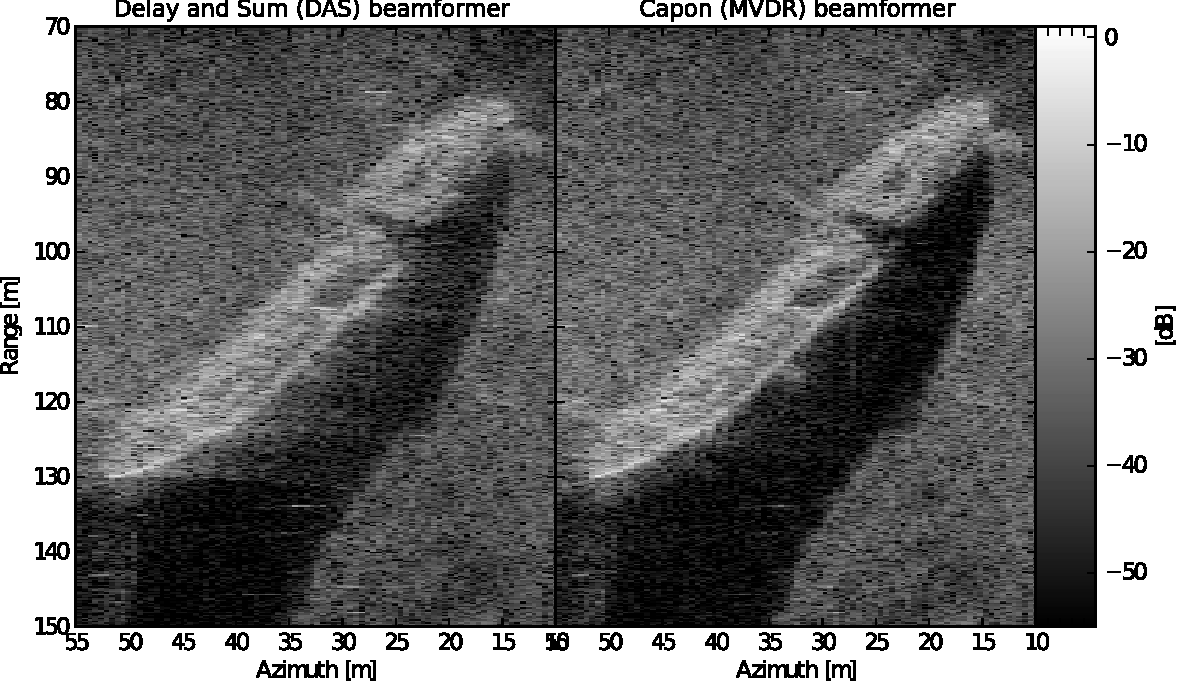
\includegraphics[width=\linewidth]{gfx/img_holmengraa.ps}
\caption{HISAS sidescan sonar (SSS) image of the shipwreck Holmengraa.}\label{holmengraa}
\end{figure}


\section{Results}

We have tested our \gls{GPU} implementation of the \gls{MVDR} beamformer on two different experimental datasets from the 32 element Kongsberg Maritime HISAS1030 sonar~\cite{Hansen2009}. The sonar was attached to the HUGIN \gls{AUV}, and one one of the datasets used in sidescan mode to image the 1500 dwt oil tanker wreck Holmengraa (\Fig{holmengraa}). Holmengraa is roughly 68\,m long and 9\,m wide, and lies on a slanted seabed at 77\,m depth. The \gls{MVDR} image was created with the parameters $L=16$, $N_\text{avg}=3$, and $d=1\%$, which proved to be a reasonable selection for this scenario.

\begin{figure}[!t]
\centering
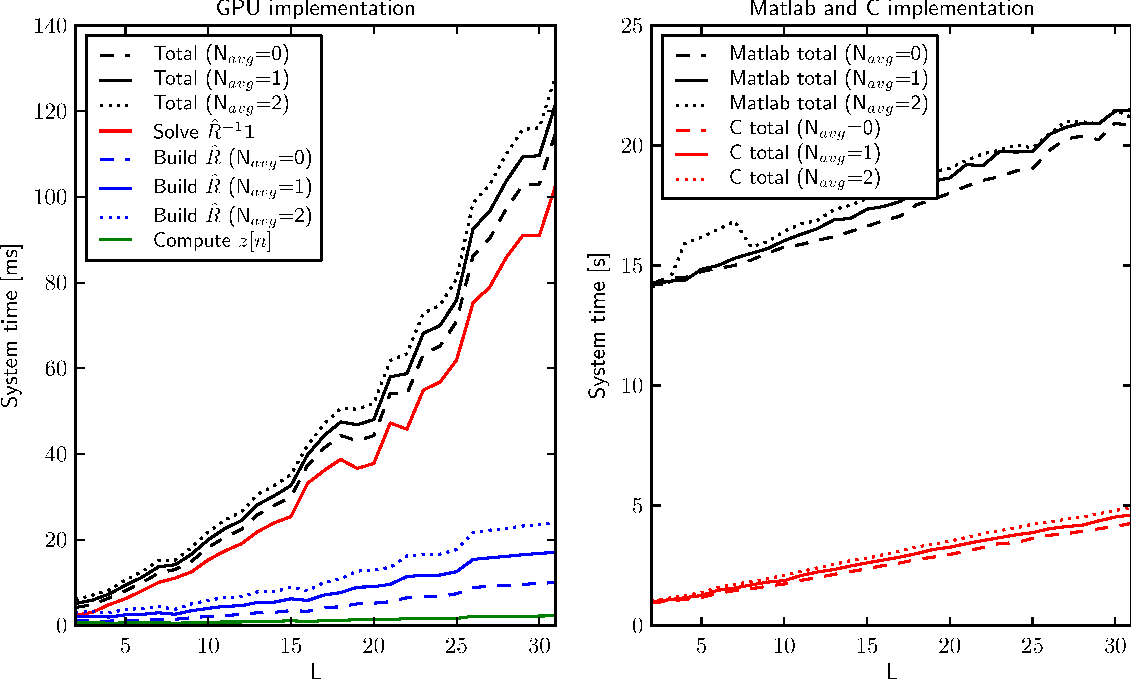
\includegraphics[width=\linewidth]{gfx/benchmark.ps}
\caption{\protect\gls{MVDR} benchmarks. Forming a 55\,kpixel image from a $M=32$ channel array.}\label{benchmarks}
\end{figure}

The other dataset was a 55\,kpixel sectorscan test image. We used it to benchmark our \gls{MVDR} implementation, and compared the result with the runtimes of an optimized single-thread C and Matlab implementation (\Fig{benchmarks}). Processing times are shown for varying subarray lengths $L$ and varying amounts of temporal averaging $N_\text{avg}$. The test system was a quad-core Intel Xeon E5620, with 64Gb of \gls{RAM}, and an nVidia Quadro 6000 card. This is a \gls{GPU} with 448 \gls{CUDA} cores and 6Gb of onboard \gls{RAM}, capable of performing roughly 1Tflops.

\section{Discussion}

Figure \ref{holmengraa} demonstrates the \gls{MVDR} beamformer's ability to suppress interference and achieve better detail resolution. Compared the \gls{DAS} beamformer, the ship's edges come out as sharper, and the shadows are less noisy. But while \gls{DAS} processed this 1.3\,Mpixel image in milliseconds, our Matlab implementation of \gls{MVDR} beamformer needed minutes.

As Figure \ref{benchmarks} illustrates, using a \gls{GPU} improves matters. If we look at the total runtimes for a subarray size of $L=16$ and $2N_\text{avg}+1=5$ pixels of temporal averaging, the \gls{GPU} implementation is able to process the test image in roughly 40\,ms. This translates to a processing throughput of 1.4\,Mpixels/s. For the same scenario the C implementation clocked in at roughly 3\,s and Matlab at 17\,s, which is 75 and 435 times slower than the \gls{GPU} implementation, respectively.

\newpage
Interesting to note is also that solving $\eRi\1$ remains the main bottleneck in the \gls{GPU} implementation, and it gets even worse for larger $L$'s. However, this is a general Gauss Jordan solver which does not exploit symmetry properties of $\eR$, so creating e.g.\ a batch based Cholesky solver should improve the runtimes further. Both the C and Matlab implementation in this benchmark take this symmetry into account, which partially explains why the complexity curves of these implementations are different from that of the \gls{GPU} implementation.

If the HISAS1030 was attached to a platform moving at 1.8m/s, for which the maximum range is 250\,m~\cite{Hansen2010}, the pulse repetition frequency could be set to 3\,Hz. We further assume a critical complex sampling frequency equal to the HISAS1030's bandwidth of 30\,kHz, and beamform $M=32$ lateral beams. The throughput required for realtime processing of these images would then be 1\,Mpixels/s. As we have seen, this is something our \gls{GPU} implementation can handle if $L$ is not too large.%, leaving the \gls{CPU} free to take on other assignments.


- Sidescan: 40kHz 

What may this performance be used for? Let us assume that the 32 element, 1.2\,m long HISAS1030 array is mounted on a platform moving at 1.8\,m/s. Then the pulse repetition frequency (PRF) could be set to 3\,Hz to ensure critical along-track sampling, 
To illustrate what this performance might be used for, consider a moving platform travelling at 1.8\,m/s. 
If the sonar system is Maximum range 
There is a limit to the along-track sampli
To avoid along track undersampling, the 

% HUGIN: 1.8m/s - range 250m \\
% fs = 100kHz*30\%*$\frac{4}{3}$ = 40kHz \\
% $N_{range px} = \frac{2\,250m}{1500m/s}40kHz = 13.3kpx$ \\
% $\times 32$ beams = 426kpx \\\\
% 
% PRF = $\frac{1500m/s}{2 250m} = 3Hz$ \\
% TP = 215px 3Hz = 1.28Mpx/s \\
% 4 arrays: 1.28Mpx/s * 4 = 5.12Mpx/s
% 
% 
% \begin{itemize}
% \item Need for speed: HUGIN 4 banks of 32 elements, can be processed faster than the ping repetition rate, with margins to spare.
% \end{itemize}


\section{Conclusion}

The \gls{MVDR} beamformer is an algorithm well suited for implementation on a \gls{GPU}. This is because the computations involved are independent on a pixel level, and partially also within each pixel. We were able to achieve speedup factors of 2-3 orders of magnitude by implementing our active sonar capable \gls{MVDR} implementation on a high-end \gls{GPU}. This performance is sufficient for computing critically sampled full-coverage sectorsscan images from the HISAS1030 sonar in realtime. Furthermore, even if such processing speeds are not required, it might be advantageous to relieve the \gls{CPU} from some of its workload. After all, these chips were designed to cooperate.


%%%%%%%%%%%%%%%%%%                              ~~~~~~~~~~~~~~~~~~~~~~~~~~~~~~~~~~~~~~~~~~~~~~~~~~
% DOCUMENT APPENDICES %
%%%%%%%%%%%%%%%%%%                              ~~~~~~~~~~~~~~~~~~~~~~~~~~~~~~~~~~~~~~~~~~~~~~~~~~


% \titleformat{<command>}[<shape>]{<format}{<label>}{<sep>}{<before>}[<after>]

% \titleformat{\section}[hang]{\bf}
% {\thesection.\enspace}%\thesubsubsection}%  {\footnotesize \enspace \emph{Sec.}  }
%    {0pt}{\MakeUppercase}[]
% \titlespacing*{\section}{0pt}{2\lineheight}{\lineheight}

% {-2ex plus -.5ex minus -.2ex}{1.0ex plus .2ex minus .2ex}

% \renewcommand\section[1]{{\Large\bf\MakeUppercase #1}}
% \renewcommand\section*[1]{{\Large\bf\MakeUppercase #1}}

\section*{Acknowledgments}

The authors would like to thank nVidia for providing them their unofficial linear equation batch solver, and Kongsberg Maritime and the Norwegian Defence Research Establishment (FFI) for providing experimental data.
% 
% 
% 
% 
% 
% 
% \section{Introduction}
% 
% \todopar{Case:
% \begin{itemize}
% \item UFFC(?)
% \item Ultrasound. Arrays up to 128 channels. Processing power vital. What's the best way to implement 
% \item Other articles evaluates Capon image quality, and some have shown that speedups can be achieved by reducing the complexity of the traditional Capon algorithm or by implementing specific versions on a GPU.
% \item This article compare a few promising ways to implement Capon in general, in light of general complexity and suitability for implementation on a CPU and GPU.
% \end{itemize}
% }
% 
% \begin{itemize}
% \item As briefly as possible, introduce beamforming.
% \item Adaptive beamformer's potential lies in its ability to suppress interference power
% \item Why adaptive beamformers struggle in active sonar systems. Correlated noise, robustification kills the adaptive potential. Quite computationally intensive. Constraints must be applied in one way or another - parameters must be tuned.
% \item The three main ways to implement Capon \cite{Capon1969} is \todo{not entirely true?}
% \begin{itemize}
% \item Traditional way: Build $\eR$ and solve $\w = \frac{\Ri\a}{\a\H\Ri\a}$. 
% \item Iterative methods: Woodbury, Conjugated gradients
% \item Beamspace
% \item LCA (or other methods, as reference)
% \end{itemize}
% \item Choice of robustification parameters $L,M,\Delta$ largely impacts what the ``optimal'' way of implementing Capon 
% \item In most imaging applications 
% Outline:
% \begin{itemize}
% \item Speeding up: Build $\eR$ and solve $\w = \frac{\Ri\a}{\a\H\Ri\a}$. 
% \item Iterative methods: Woodbury (Sherman Morrison), Conjugated gradients - show performance of GPU performance.
% \item Woodbury: Must take the average over many samples in space and time - lots of (small) outerproducts. Can be used if not a lot of averaging is required.
% \item Beamspace
% \item LCA (or other methods, as reference)
% \end{itemize}
% \end{itemize}
% 
% fs = 100kHz*30\%*$\frac{4}{3}$ = 40kHz \\
% $N_{range px} = \frac{2\,250m}{1500m/s}40kHz = 13.3kpx$ \\
% $\times 32$ beams = 426kpx \\\\
% 
% PRF = $\frac{1500m/s}{2 250m} = 3Hz$ \\
% TP = 215px 3Hz = 1.28Mpx/s \\
% 4 arrays: 1.28Mpx/s * 4 = 5.12Mpx/s
% 
% 
% \section{Methods}
% 
% \begin{align}
% z[n] = \sumb{m=0}{M-1} w_m[n]^*x_m[n-\Delta_m] = \w\H[n]\Xd[n]
% \end{align}
% where
% \begin{align}
% \w[n] = \bmat{w_0[n]\\w_1[n]\\\vdots\\w_{M-1}[n]} \quad \text{and} \quad\Xd[n] = \bmat{x_0[n]\\x_1[n]\\\vdots\\x_{M-1}[n]}.
% \end{align}
% 
% Minimum variance distortionless resonse \cite{Capon1969}
% \begin{align}
% \underset{\w[n]}{\argmin}\, E\{ |z[n]|^2 \} = \underset{\w[n]}{\argmin}\, \w\H[n]\R[n]\w[n], 
% \end{align}
% subject to
% \begin{align}
% \w\H[n]\a = 1,
% \end{align}
% where
% \begin{align}
% \R[n] = E\{ \x\x\H \}.
% \end{align}
% If $\eR$ is the estimate of $\R$, the solution to the MVDR beamformer is
% \begin{gather*}
% \vec w[n] = \frac{\hat{\mat R}\,\!^{-1}[n]\vec a}{\vec a\H\hat{\mat R}\,\!^{-1}[n]\vec a} = \frac{\text{\raisebox{1.9pt}{$\vec\chi$}}[n]}{\vec a\H\text{\raisebox{1.9pt}{$\vec\chi$}}[n]}
% \end{gather*}
% A robust estimate of $\eR$ is found by
% \begin{itemize}
% \item Spatial averaging to decorrelate noise from signal. \emph{Subarray averaging} used here.
% \item Temporal averaging to ensure valid speckle statistics.
% \item \emph{Diagonal loading} to ensure  numerical stability prior to inversion.
% \item Choice of robustification parameters \cite{Synnevag2007}
% \end{itemize}
% 


\newpage
Here $\vec a$ is a \emph{steering vector} that if set to $\vec 1$ steers towards broadside, and $\hat{\mat R}$ is an estimate of the spatial covariance matrix, often computed as
\begin{gather*}
r_{ij}[n] = \frac{1}{K(2N_{\text{avg}}+1)}\sumb{k=0}{K-1} \sumb{n'=n-N_{\text{avg}}}{n+N_{\text{avg}}} x_{i+k}[n']\,x_{j+k}[n'],
\end{gather*}
where $r_{ij}$ is the $(i,j)$'th element of the covariance matrix, $K$ is the number of subarrays, $2N_{\text{avg}}+1$ is the number of samples to perform time averaging over, and $\vec x_i[n']$ is the data recorded by the $i$'th sensor at sample $n'$. 



{\bf Method complexity (instructions):}\\
\begin{tabular}{l l}
No optimizations            & $2M^2\,(2\Navg+1)$ \\
Banded symmetric            & $L(2M-L+1)\,(2\Navg+1)$ \\
Sliding, banded, symmetric  & $1.5L(2M-L+1)$ \\
\end{tabular}\\\\


% 
% \subsubsection{Computing $\text{\raisebox{1.9pt}{$\vec\chi$}} = \hat{\mat R}\,\!^{-1}\vec a$}
% 
% There are two ways of finding $\text{\raisebox{1.9pt}{$\vec\chi$}} = \hat{\mat R}\,\!^{-1}\vec a$, either by solving the equation directly or by inverting $\hat{\mat R}$ first. Solving the equation is less computationally intensive than inverting $\hat{\mat R}$, and seems like the obvious choice. However, with iterative methods for updating $\eRi$ for each range pixel the situation is changed...

% 
% \subsection{Iterative methods}
% 
% \begin{itemize}
% \item Woodbury
% \item Conjugated gradients
% \end{itemize}
% 
% 
% \subsection{Beamspace}
% 
% \begin{itemize}
% \item Some minimum of background, and good references.
% \end{itemize}
% 
% 
% \section{Results/Discussion}
% 
% 
% 
% 
% 
% \begin{itemize}
% \item Compare computational complexity vs. memory constraints for the various methods. Supporting plots.
% \item Relate this to whether the favourable architecture is a CPU or a GPU \todo{check ``when to gpu article''}
% \item Run benchmarks on some sonar dataset(s)
% \end{itemize}
% 
% 
% \section{Conclusion}
% 
% \begin{itemize}
% \item When to use what.
% \end{itemize}
% 
% 
% % \ \\
% % \IEEEPARstart{T}{o} form images from a modern phased array sonar system the received wavefield is usually recorded, and then postprocessed by a digital beamformer. The beamformer applies delays and weights to the sensor channels, the beamformer adjusts the arrays spatial response to focus at one pixel at a time.  such that signals emanating from regions of interest add constructively, while ensuring that noise and interference from other angles do not. 
% % 
% % The imaging capabilities of a modern phased array sonar system depend on physical attributes such element response and array geometry, the transmitted signal, as well as the beamforming method being used on transmission and reception. Beamforming is the concept of applying delays and weights to the sensors channels to steer the arrays response to points of interest. 
% 
% % 
% % 
% % Outline:
% % \begin{itemize}
% % \item Capon's resonse when applying robustification
% % \item Choice of window functions makes little difference.
% % \item Steering and mainlobewidths have outer bounds.
% % \item Beamspace?
% % \item Chosen window plots - what may they tell us? Variance intensity values when using various windows.
% % \item Assymmetric windows?
% % \end{itemize}
% % 
% % 
% % \begin{align}
% % z[n] = \sumb{m=0}{M-1} w_m[n]^*x_m[n-\Delta_m] = \w\H[n]\x[n-\Delta_m]
% % \end{align}
% % 
% % 
% % \section{Methods}
% % 
% % Basically, we are working with a practical implementation of the Capon beamformer that computes a set of weights $\vec w$ for every single sample $n$ by solving:
% % \begin{gather*}
% % \vec w[n] = \frac{\hat{\mat R}\,\!^{-1}[n]\vec a}{\vec a\H\hat{\mat R}\,\!^{-1}[n]\vec a} = \frac{\text{\raisebox{1.9pt}{$\vec\chi$}}[n]}{\vec a\H\text{\raisebox{1.9pt}{$\vec\chi$}}[n]}
% % \end{gather*}%
% % where
% % % \newcommand\X{\text{\raisebox{2pt}{$\vec\chi$}}}
% % \begin{gather*}
% % \text{\raisebox{1.9pt}{$\vec\chi$}} = \hat{\mat R}\,\!^{-1}\vec a \qquad\qquad\text{is the solution to}\qquad\qquad \hat{\mat R}\text{\raisebox{1.9pt}{$\vec\chi$}} = \vec a.
% % \end{gather*}
% 
% % 
% % , and maximum suppression of while ensuring that the beamformer digitally  before each of the pixels are estimated one at a time. The resolution and contrast of such a system will depend on the systems spatial response, which ideally should be narrow  be very sharp in the desired direction its ability to achieve  fundamental principle of forming a sonar image is to record the received wavefield, 
% % 
% % image quality of a phased array sonar imaging systems depend on  the choice of weights to apply to each of the sensors are crucial. 
% % 
% % A modern phased array imaging system may be thought of as a spatial filter. To achieve the best possible performance, the 
% % 
% % resolution and contrast 
% % 
% % Adaptive beamformers have only recently been introduced in active sonar imaging. For a while they were considered unsuited for this purpose because the backscattered signal is largely correlated with the 
% % 
% % 
% % 
% 
% %\begin{figure}[!t]
% %\centering
% %\includegraphics[width=2.5in]{myfigure}
% % where an .eps filename suffix will be assumed under latex, 
% % and a .pdf suffix will be assumed for pdflatex; or what has been declared
% % via \DeclareGraphicsExtensions.
% %\caption{Simulation Results}
% %\label{fig_sim}
% %\end{figure}
% 
% 
% % An example of a double column floating figure using two subfigures.
% % (The subfig.sty package must be loaded for this to work.)
% % The subfigure \label commands are set within each subfloat command, the
% % \label for the overall figure must come after \caption.
% % \hfil must be used as a separator to get equal spacing.
% % The subfigure.sty package works much the same way, except \subfigure is
% % used instead of \subfloat.
% %
% % \begin{figure*}[!t]
% % \centerline{\subfloat[Case I]\includegraphics[width=2.5in]{subfigcase1}%
% % \label{fig_first_case}}
% % \hfil
% % \subfloat[Case II]{\includegraphics[width=2.5in]{subfigcase2}%
% % \label{fig_second_case}}}
% % \caption{Simulation results}
% % \label{fig_sim}
% % \end{figure*}
% %
% % Note that often IEEE papers with subfigures do not employ subfigure
% % captions (using the optional argument to \subfloat), but instead will
% % reference/describe all of them (a), (b), etc., within the main caption.
% 
% 
% % An example of a floating table. Note that, for IEEE style tables, the 
% % \caption command should come BEFORE the table. Table text will default to
% % \footnotesize as IEEE normally uses this smaller font for tables.
% % The \label must come after \caption as always.
% %
% %\begin{table}[!t]
% %% increase table row spacing, adjust to taste
% %\renewcommand{\arraystretch}{1.3}
% % if using array.sty, it might be a good idea to tweak the value of
% % \extrarowheight as needed to properly center the text within the cells
% %\caption{An Example of a Table}
% %\label{table_example}
% %\centering
% %% Some packages, such as MDW tools, offer better commands for making tables
% %% than the plain LaTeX2e tabular which is used here.
% %\begin{tabular}{|c||c|}
% %\hline
% %One & Two\\
% %\hline
% %Three & Four\\
% %\hline
% %\end{tabular}
% %\end{table}
% 
% 
% % Note that IEEE does not put floats in the very first column - or typically
% % anywhere on the first page for that matter. Also, in-text middle ("here")
% % positioning is not used. Most IEEE journals use top floats exclusively.
% % However, Computer Society journals sometimes do use bottom floats - bear
% % this in mind when choosing appropriate optional arguments for the
% % figure/table environments.
% % Note that, LaTeX2e, unlike IEEE journals, places footnotes above bottom
% % floats. This can be corrected via the \fnbelowfloat command of the
% % stfloats package.
% 
% 
% 
% \section{Conclusion}
% The conclusion goes here.
% 
% 
% 


% if have a single appendix:
%\appendix[Proof of the Zonklar Equations]
% or
%\appendix  % for no appendix heading
% do not use \section anymore after \appendix, only \section*
% is possibly needed

% use appendices with more than one appendix
% then use \section to start each appendix
% you must declare a \section before using any
% \subsection or using \label (\appendices by itself
% starts a section numbered zero.)
%

%%%%%%%%%%%%%%%%%%                              ~~~~~~~~~~~~~~~~~~~~~~~~~~~~~~~~~~~~~~~~~~~~~~~~~~
% DOCUMENT APPENDICES %
%%%%%%%%%%%%%%%%%%                              ~~~~~~~~~~~~~~~~~~~~~~~~~~~~~~~~~~~~~~~~~~~~~~~~~~

\appendices



% use section* for acknowledgement
\ifCLASSOPTIONcompsoc
  \section*{Acknowledgments}
\else
  \section*{Acknowledgment}
\fi


The authors would like to thank...


% Can use something like this to put references on a page
% by themselves when using endfloat and the captionsoff option.
\ifCLASSOPTIONcaptionsoff
  \newpage
\fi



% trigger a \newpage just before the given reference
% number - used to balance the columns on the last page
% adjust value as needed - may need to be readjusted if
% the document is modified later
%\IEEEtriggeratref{8}
% The "triggered" command can be changed if desired:
%\IEEEtriggercmd{\enlargethispage{-5in}}

% references section

\bibliographystyle{IEEEtran}
\bibliography{../../Library/library}

% End up doing this:
% \begin{thebibliography}{1}
% 
% \bibitem{IEEEhowto:kopka}
% H.~Kopka and P.~W. Daly, \emph{A Guide to {\LaTeX}}, 3rd~ed.\hskip 1em plus
%   0.5em minus 0.4em\relax Harlow, England: Addison-Wesley, 1999.
% 
% \end{thebibliography}



% biography section
% 
% If you have an EPS/PDF photo (graphicx package needed) extra braces are
% needed around the contents of the optional argument to biography to prevent
% the LaTeX parser from getting confused when it sees the complicated
% \includegraphics command within an optional argument. (You could create
% your own custom macro containing the \includegraphics command to make things
% simpler here.)
%\begin{biography}[{\includegraphics[width=1in,height=1.25in,clip,keepaspectratio]{mshell}}]{Michael Shell}
% or if you just want to reserve a space for a photo:

\vfill 

\begin{IEEEbiography}{Noname dude}
He doesn't exist.
\end{IEEEbiography}

% if you will not have a photo at all:
\begin{IEEEbiographynophoto}{Jo Inge Buskenes}
Not in at the moment.
\end{IEEEbiographynophoto}

%\newpage

% \begin{IEEEbiographynophoto}{Jo Inge Buskenes}
% Not in at the moment.
% \end{IEEEbiographynophoto}

%\vfill

% Can be used to pull up biographies so that the bottom of the last one
% is flush with the other column.
%\enlargethispage{-5in}

\markboth{}%
{}
% \newpage
\begin{figure*}[!t]
\begin{narrow}{-1.2cm}{-1.2cm}\centering\vspace{-1.0cm}
\textbf{1. LCA with trigonometric and Kaiser windows - Capon shining}\\
\begin{tabular}[c]{l l l l}
\bf General & M = 32                            & $\Delta r = \frac{c}{2B}$ = 2.5 cm & $\frac{640\,\text{pixels}] / 12\,\text{m}}{\Delta r} = \frac{4}{3}$ \\
\bf LCA     & $\beta \in [0,10]$ (9 values) & $\phi \in [-1.07,1.07]$ deg (9 values) & Navg = 3 \\
\bf Capon   & $\Delta$ = 0.01                 & L = 16                           & Navg = 3 \\
\end{tabular}
\subfloat[LCA Window Response]{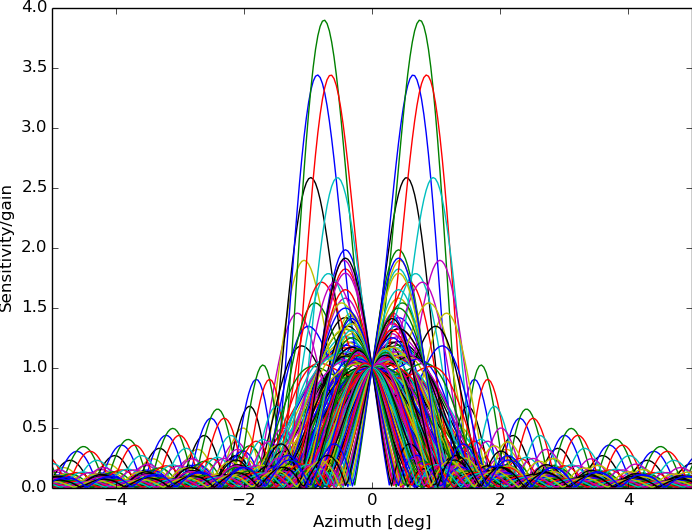
\includegraphics[width=0.49\linewidth]{gfx/1_window_response.png}}\hfill
\subfloat[Mean images]{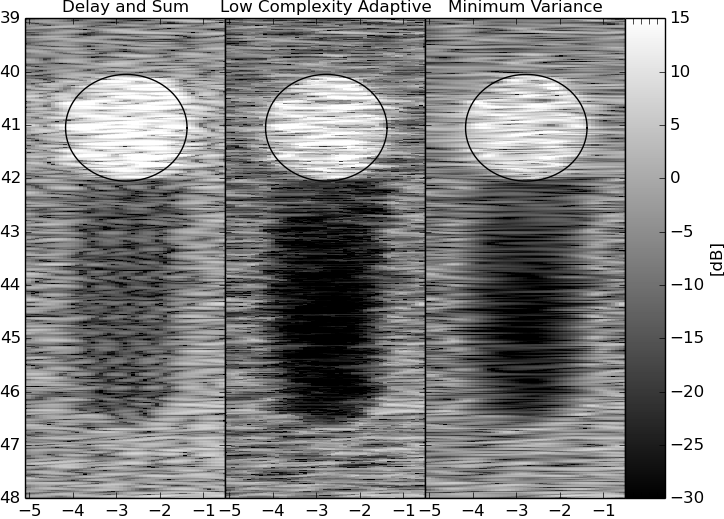
\includegraphics[width=0.49\linewidth]{gfx/1_mean_imgs.png}}\\
\subfloat[Windows ($\beta$)]{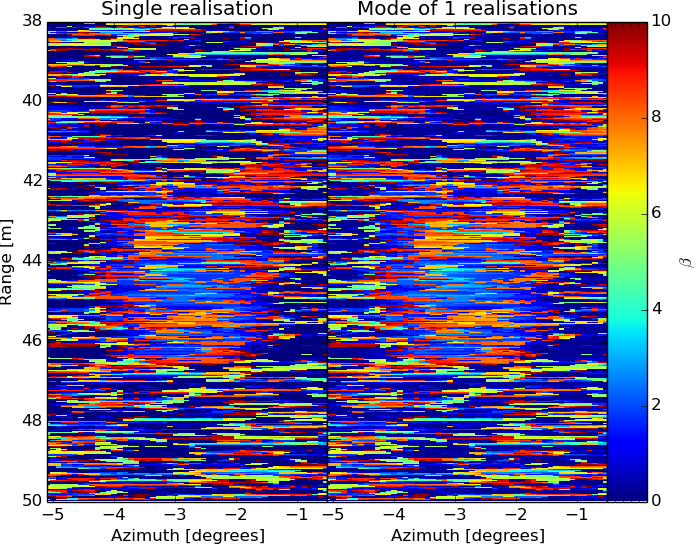
\includegraphics[width=0.49\linewidth]{gfx/1_windows_beta.png}}\hfill
\subfloat[Windows ($\phi$)]{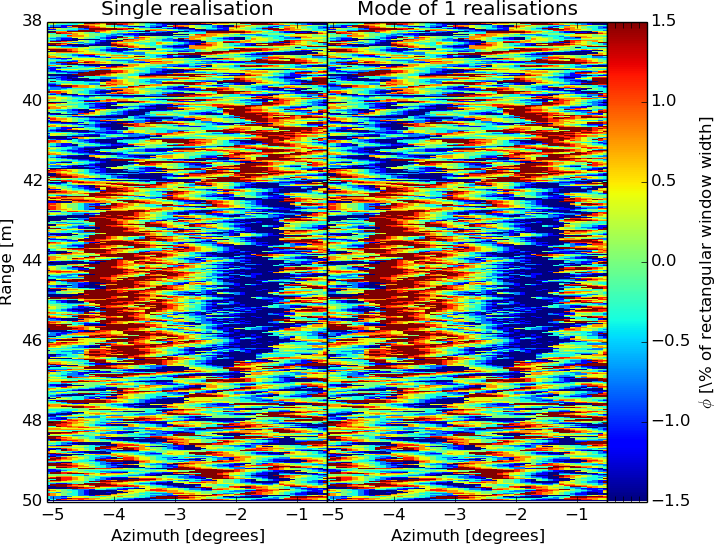
\includegraphics[width=0.48\linewidth]{gfx/1_windows_phi.png}}\\
\subfloat[Capon win. resp. through shadow]{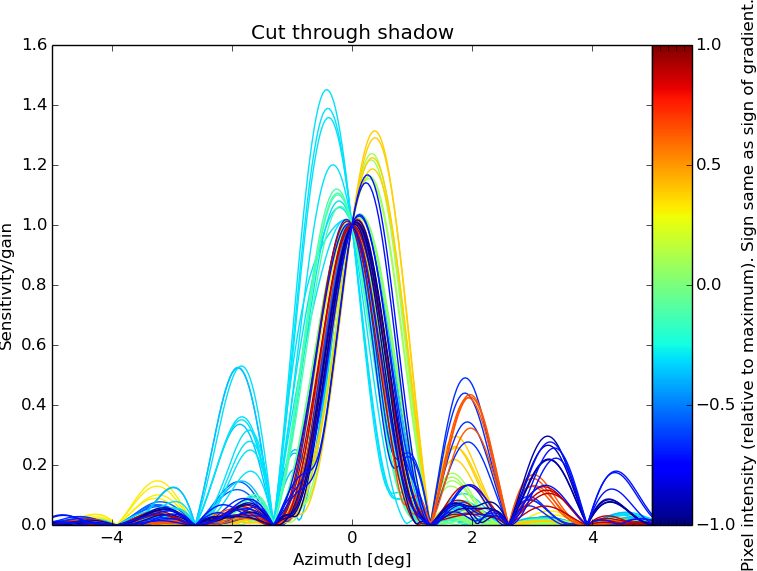
\includegraphics[width=0.49\linewidth]{gfx/1_win_resp_cut_shadow.png}}\hfill
\subfloat[Capon win. resp. through highlight]{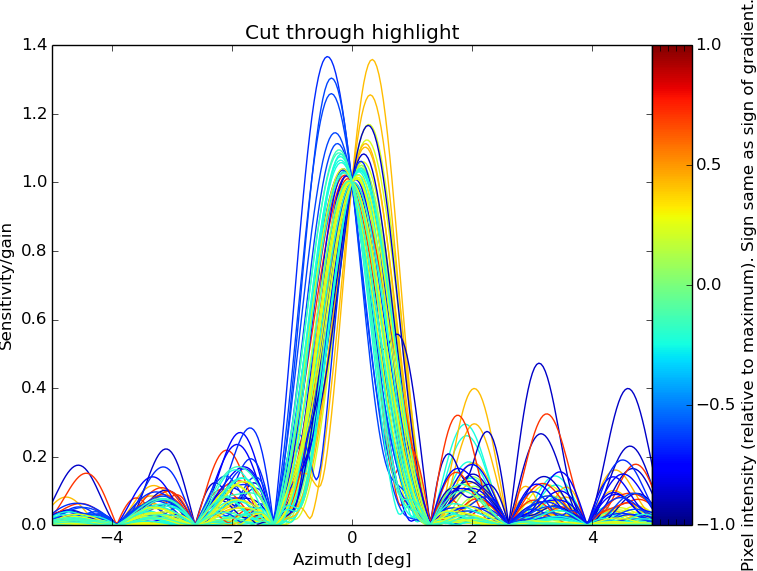
\includegraphics[width=0.49\linewidth]{gfx/1_win_resp_cut_highlight.png}}\\
\end{narrow}
\end{figure*}
\newpage
\begin{figure*}[!t]
\begin{narrow}{-1.2cm}{-1.2cm}\centering\vspace{-1.0cm}
\textbf{2. Capon: Tuning regularisation.}\\
\begin{tabular}[c]{l l l l}
\bf General & M = 32                            & $\Delta r = \frac{c}{2B}$ = 2.5 cm & $\frac{640\,\text{pixels}] / 12\,\text{m}}{\Delta r} = \frac{4}{3}$ \\
\bf LCA     & $\beta \in [0,10]$ (9 values) & $\phi \in [-1.07,1.07]$ deg (9 values) & Navg = 3 \\
\bf Capon   & $\Delta$ = 0.05                 & L = 16                           & Navg = 3 \\
\end{tabular}
\subfloat[LCA Window Response]{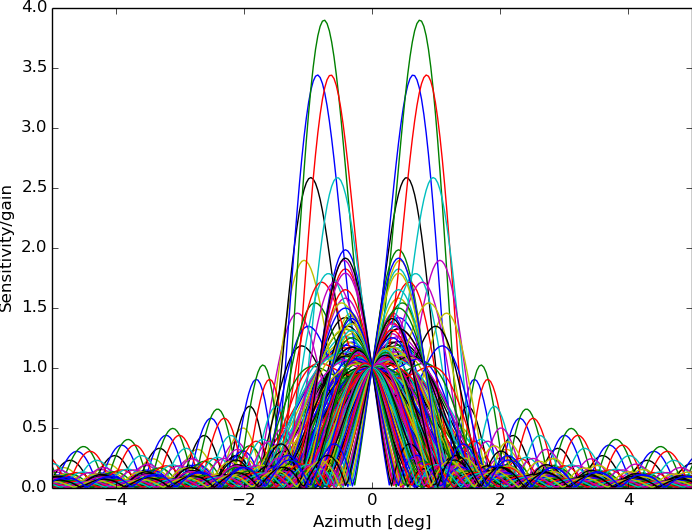
\includegraphics[width=0.49\linewidth]{gfx/2_window_response.png}}\hfill
\subfloat[Mean images]{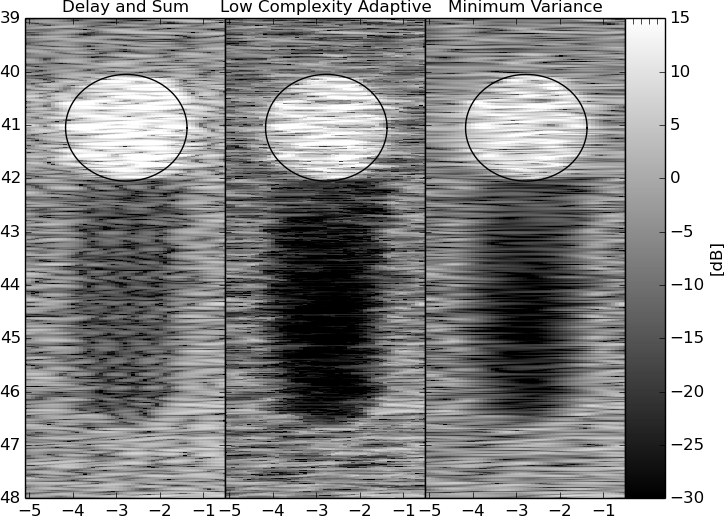
\includegraphics[width=0.49\linewidth]{gfx/2_mean_imgs.png}}\\
\subfloat[Windows ($\beta$)]{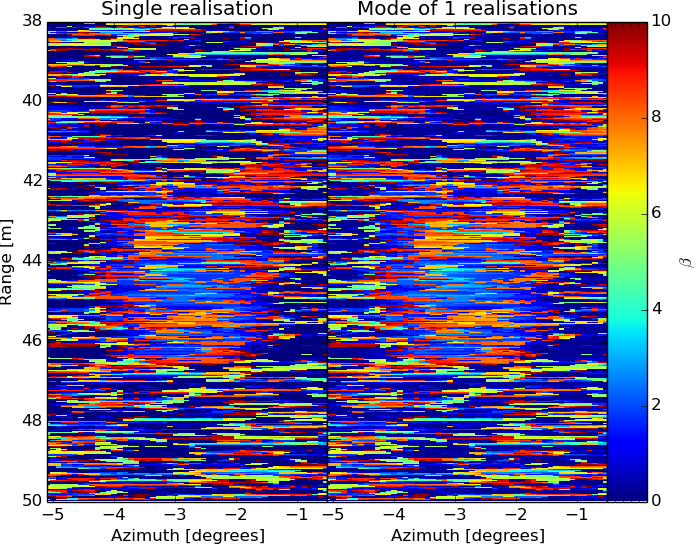
\includegraphics[width=0.49\linewidth]{gfx/2_windows_beta.png}}\hfill
\subfloat[Windows ($\phi$)]{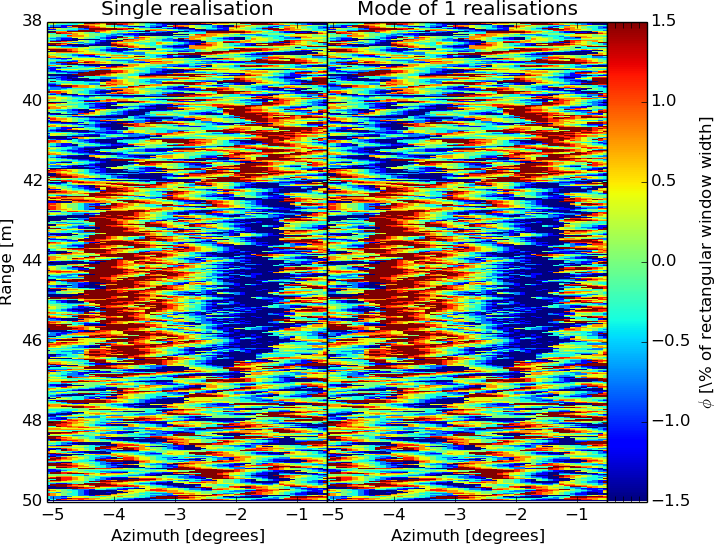
\includegraphics[width=0.48\linewidth]{gfx/2_windows_phi.png}}\\
\subfloat[Capon win. resp. through shadow]{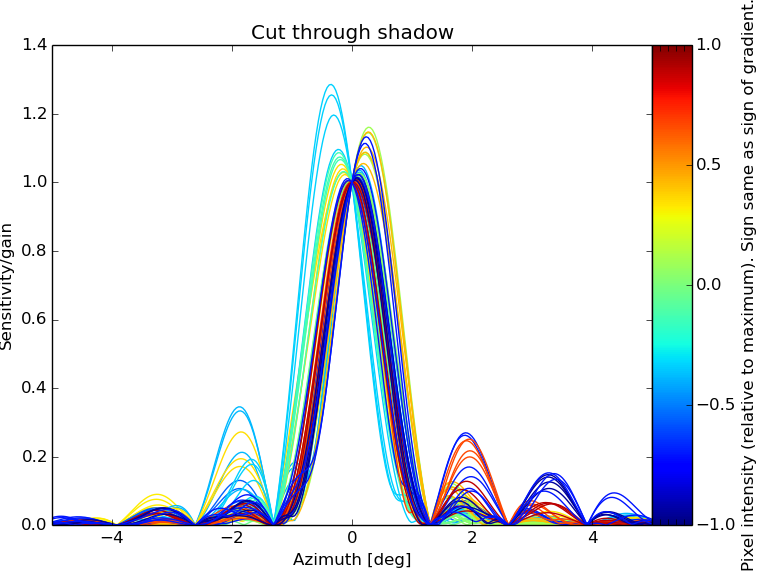
\includegraphics[width=0.49\linewidth]{gfx/2_win_resp_cut_shadow.png}}\hfill
\subfloat[Capon win. resp. through highlight]{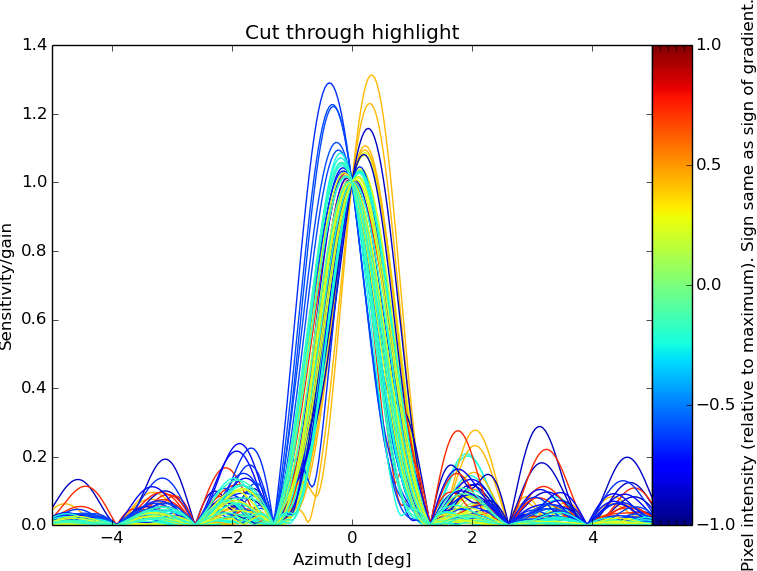
\includegraphics[width=0.49\linewidth]{gfx/2_win_resp_cut_highlight.png}}\\
\end{narrow}
\end{figure*}
\newpage
\begin{figure*}[!t]
\begin{narrow}{-1.2cm}{-1.2cm}\centering\vspace{-1.0cm}
\textbf{3. Capon: Tuning regularisation.}\\
\begin{tabular}[c]{l l l l}
\bf General & M = 32                            & $\Delta r = \frac{c}{2B}$ = 2.5 cm & $\frac{640\,\text{pixels}] / 12\,\text{m}}{\Delta r} = \frac{4}{3}$ \\
\bf LCA     & $\beta \in [0,10]$ (9 values) & $\phi \in [-1.07,1.07]$ deg (9 values) & Navg = 3 \\
\bf Capon   & $\Delta$ = 0.20                 & L = 16                           & Navg = 3 \\
\end{tabular}
\subfloat[LCA Window Response]{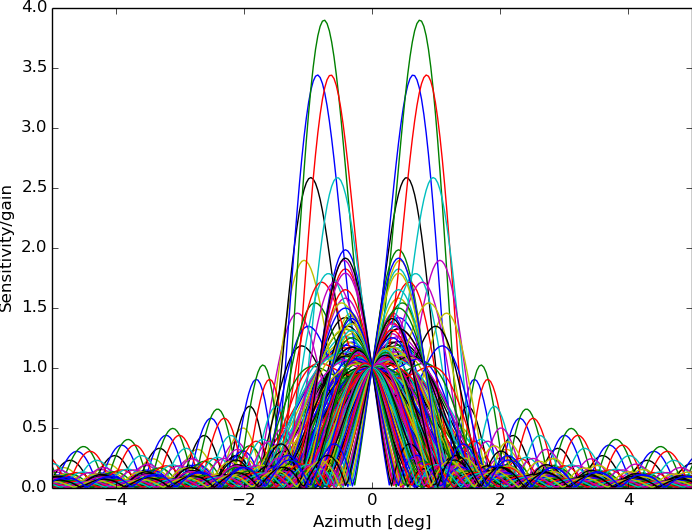
\includegraphics[width=0.49\linewidth]{gfx/3_window_response.png}}\hfill
\subfloat[Mean images]{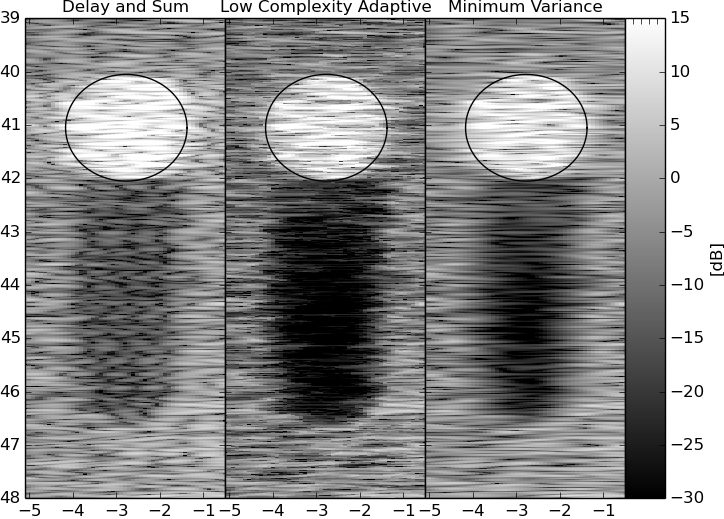
\includegraphics[width=0.49\linewidth]{gfx/3_mean_imgs.png}}\\
\subfloat[Windows ($\beta$)]{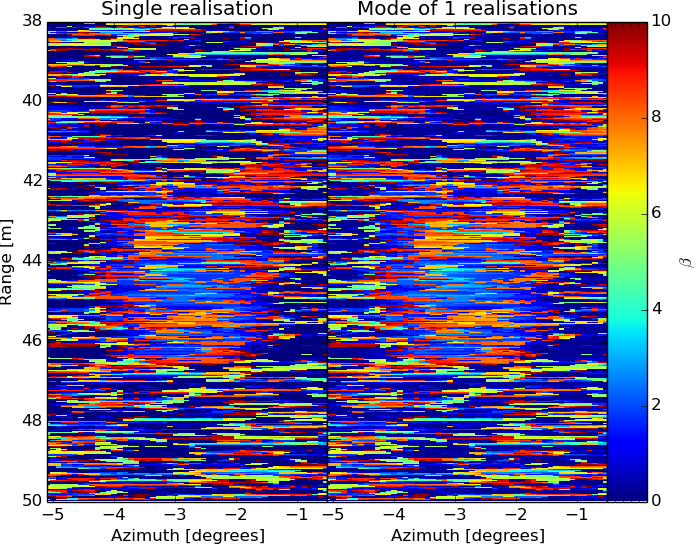
\includegraphics[width=0.49\linewidth]{gfx/3_windows_beta.png}}\hfill
\subfloat[Windows ($\phi$)]{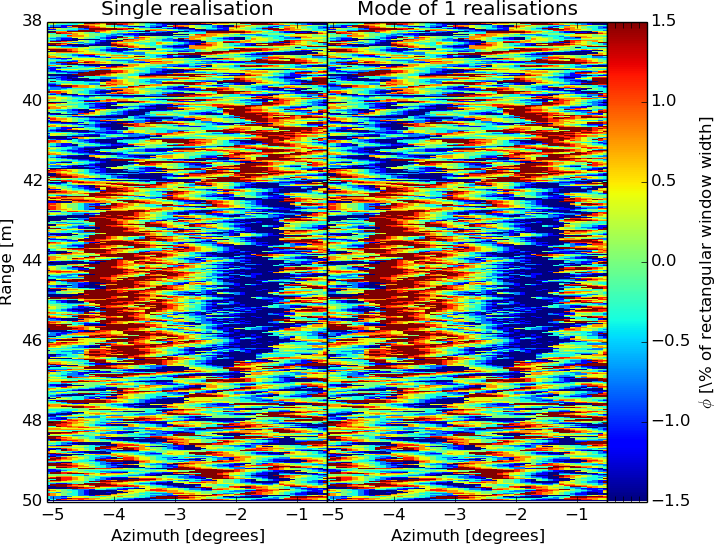
\includegraphics[width=0.48\linewidth]{gfx/3_windows_phi.png}}\\
\subfloat[Capon win. resp. through shadow]{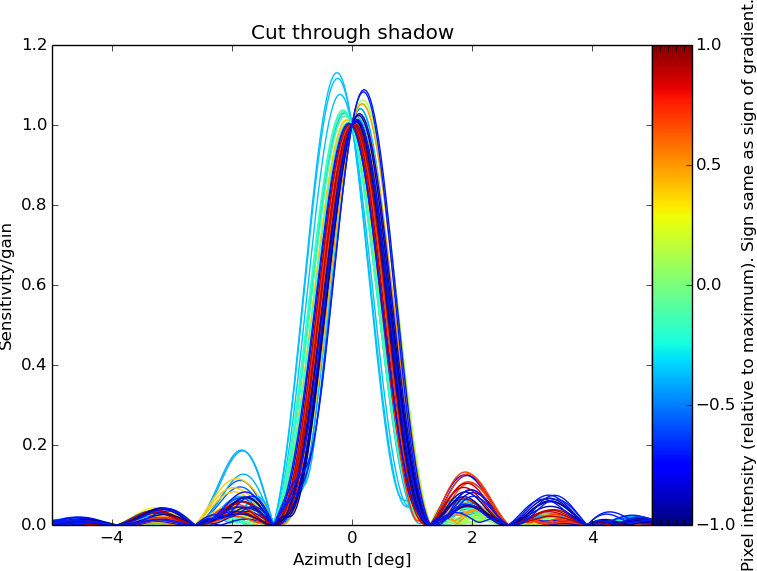
\includegraphics[width=0.49\linewidth]{gfx/3_win_resp_cut_shadow.png}}\hfill
\subfloat[Capon win. resp. through highlight]{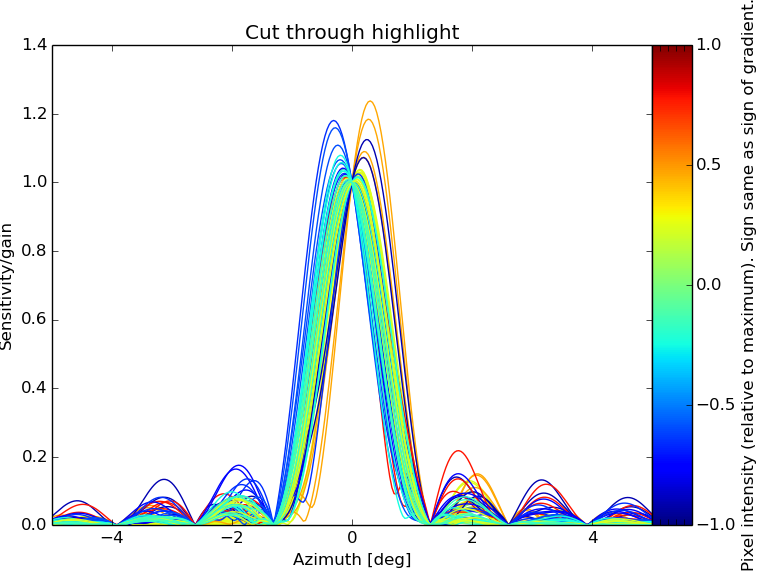
\includegraphics[width=0.49\linewidth]{gfx/3_win_resp_cut_highlight.png}}\\
\end{narrow}
\end{figure*}
\newpage
\begin{figure*}[!t]
\begin{narrow}{-1.2cm}{-1.2cm}\centering\vspace{-1.0cm}
\textbf{4. Capon: Tuning subarray.}\\
\begin{tabular}[c]{l l l l}
\bf General & M = 32                            & $\Delta r = \frac{c}{2B}$ = 2.5 cm & $\frac{640\,\text{pixels}] / 12\,\text{m}}{\Delta r} = \frac{4}{3}$ \\
\bf LCA     & $\beta \in [0,10]$ (9 values) & $\phi \in [-1.07,1.07]$ deg (9 values) & Navg = 3 \\
\bf Capon   & $\Delta$ = 0.01                 & L = 20                           & Navg = 3 \\
\end{tabular}
\subfloat[LCA Window Response]{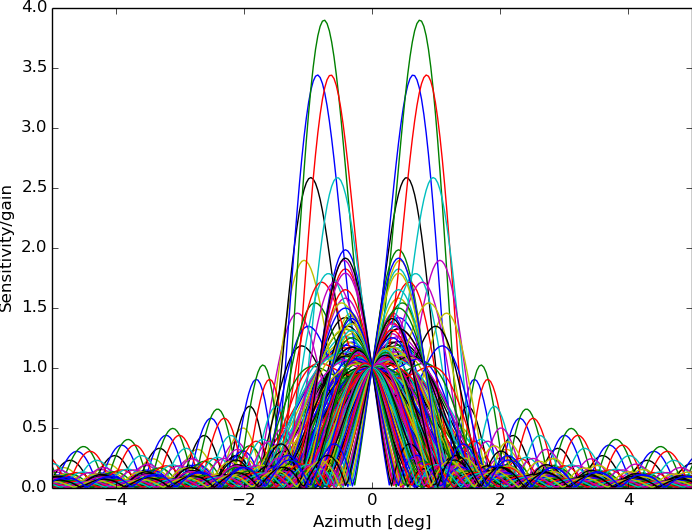
\includegraphics[width=0.49\linewidth]{gfx/4_window_response.png}}\hfill
\subfloat[Mean images]{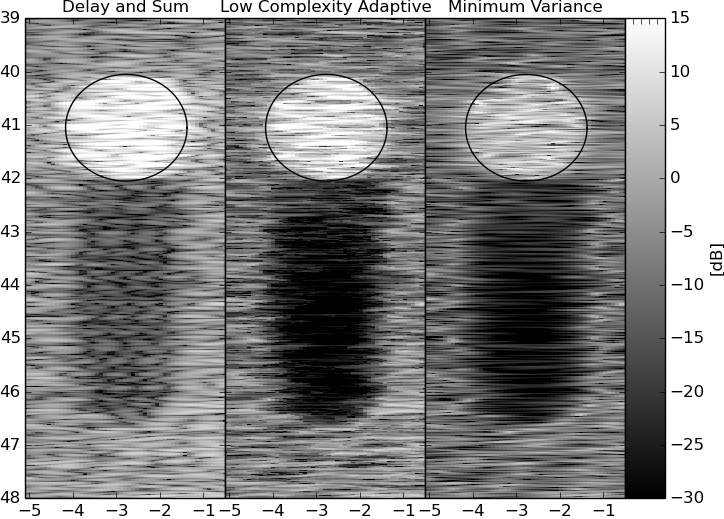
\includegraphics[width=0.49\linewidth]{gfx/4_mean_imgs.png}}\\
\subfloat[Windows ($\beta$)]{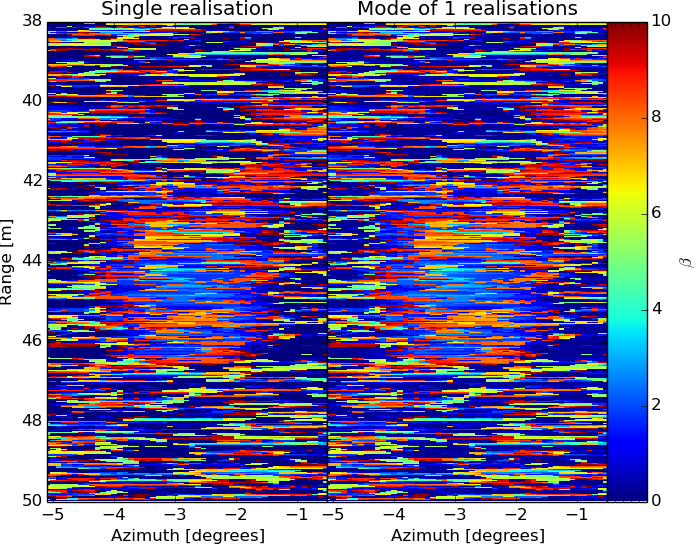
\includegraphics[width=0.49\linewidth]{gfx/4_windows_beta.png}}\hfill
\subfloat[Windows ($\phi$)]{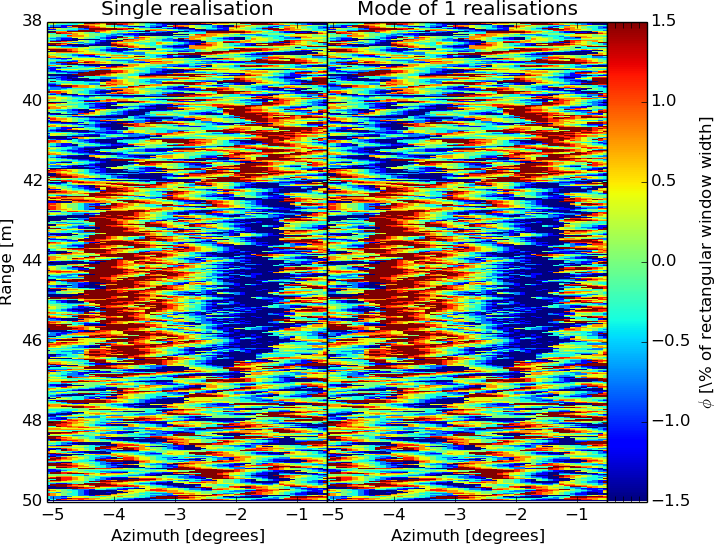
\includegraphics[width=0.48\linewidth]{gfx/4_windows_phi.png}}\\
\subfloat[Capon win. resp. through shadow]{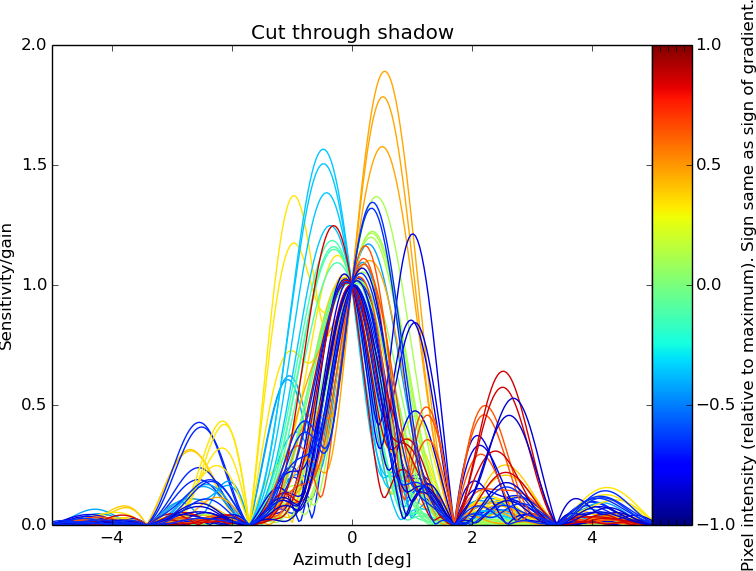
\includegraphics[width=0.49\linewidth]{gfx/4_win_resp_cut_shadow.png}}\hfill
\subfloat[Capon win. resp. through highlight]{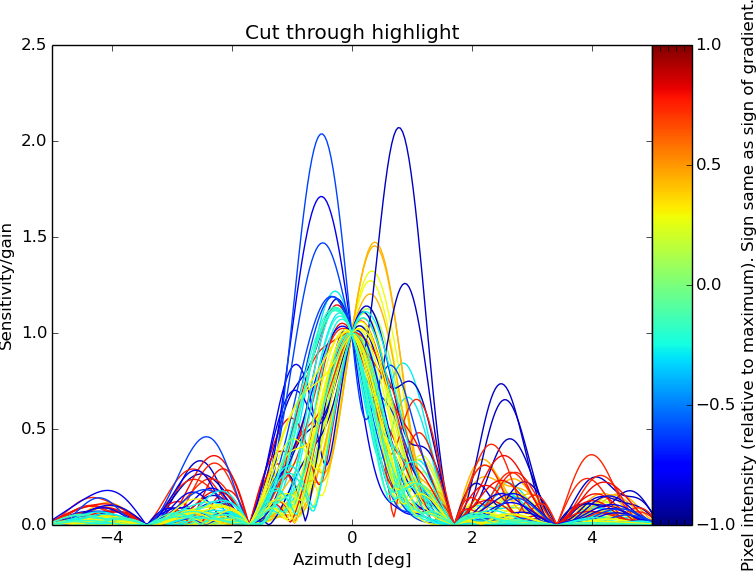
\includegraphics[width=0.49\linewidth]{gfx/4_win_resp_cut_highlight.png}}\\
\end{narrow}
\end{figure*}
\newpage
\begin{figure*}[!t]
\begin{narrow}{-1.2cm}{-1.2cm}\centering\vspace{-1.0cm}
\textbf{5. Capon: Tuning subarray.}\\
\begin{tabular}[c]{l l l l}
\bf General & M = 32                            & $\Delta r = \frac{c}{2B}$ = 2.5 cm & $\frac{640\,\text{pixels}] / 12\,\text{m}}{\Delta r} = \frac{4}{3}$ \\
\bf LCA     & $\beta \in [0,10]$ (9 values) & $\phi \in [-1.07,1.07]$ deg (9 values) & Navg = 3 \\
\bf Capon   & $\Delta$ = 0.01                 & L = 16                           & Navg = 3 \\
\end{tabular}
\subfloat[LCA Window Response]{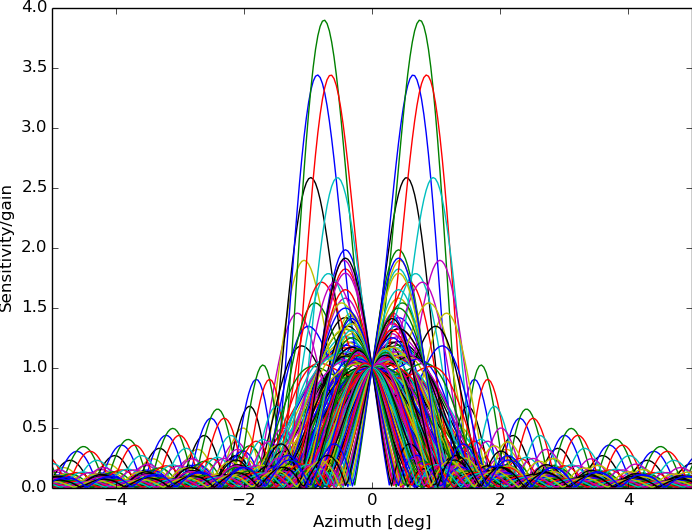
\includegraphics[width=0.49\linewidth]{gfx/5_window_response.png}}\hfill
\subfloat[Mean images]{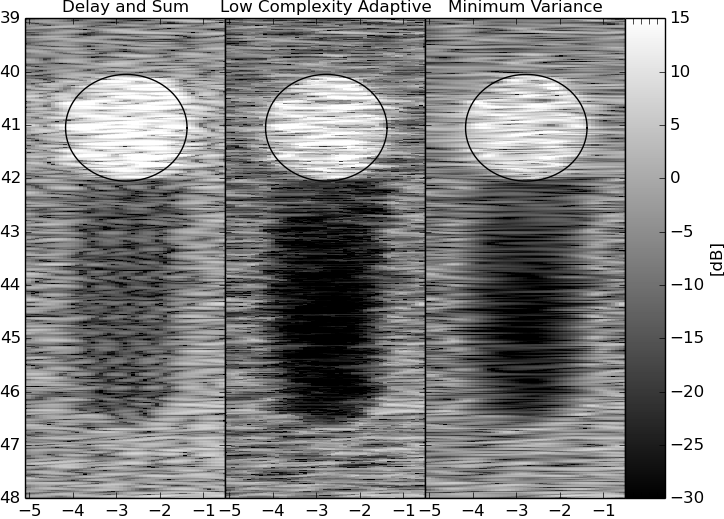
\includegraphics[width=0.49\linewidth]{gfx/5_mean_imgs.png}}\\
\subfloat[Windows ($\beta$)]{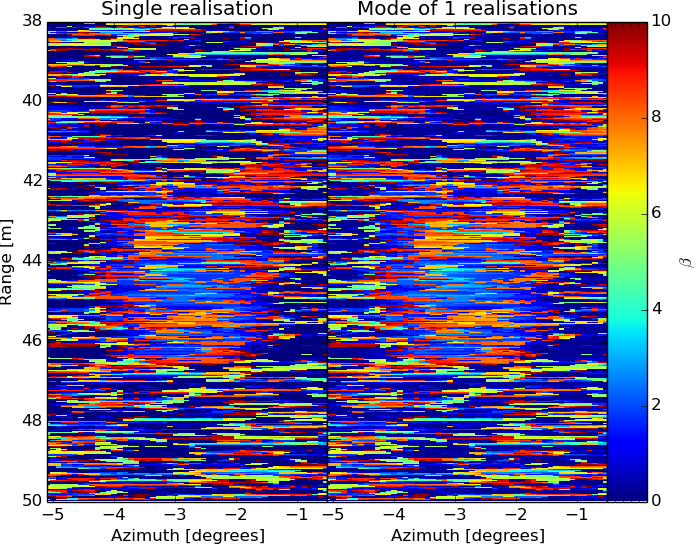
\includegraphics[width=0.49\linewidth]{gfx/5_windows_beta.png}}\hfill
\subfloat[Windows ($\phi$)]{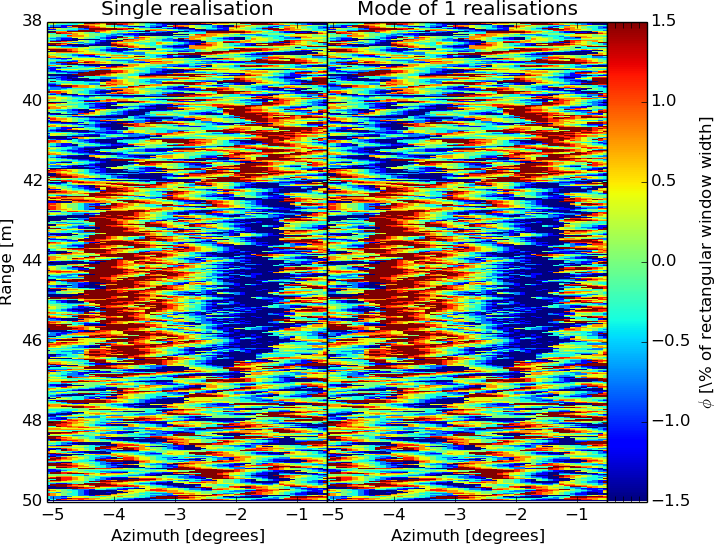
\includegraphics[width=0.48\linewidth]{gfx/5_windows_phi.png}}\\
\subfloat[Capon win. resp. through shadow]{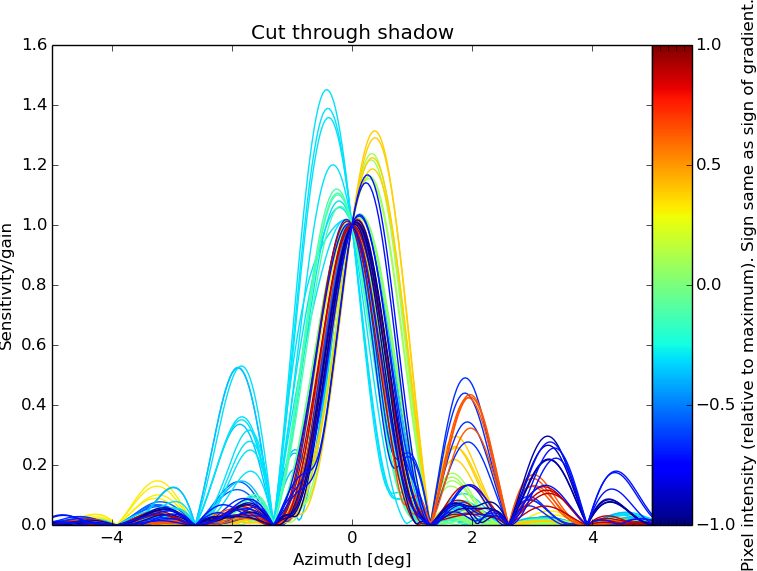
\includegraphics[width=0.49\linewidth]{gfx/5_win_resp_cut_shadow.png}}\hfill
\subfloat[Capon win. resp. through highlight]{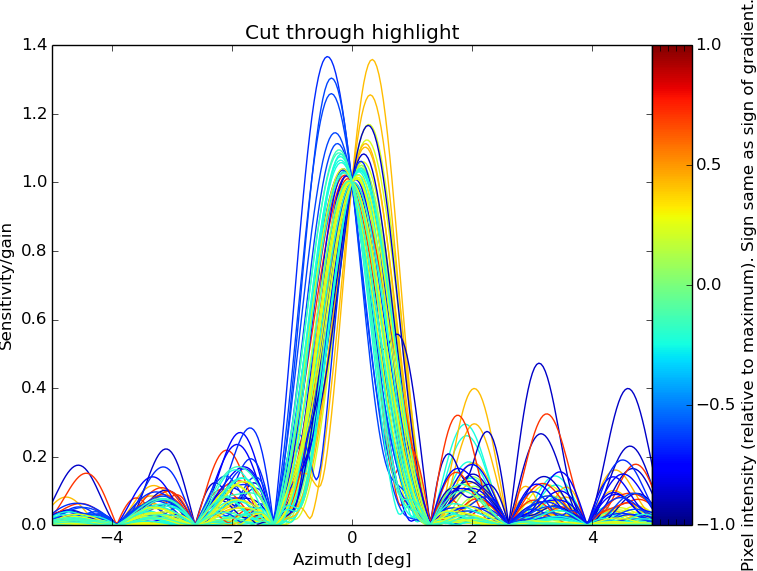
\includegraphics[width=0.49\linewidth]{gfx/5_win_resp_cut_highlight.png}}\\
\end{narrow}
\end{figure*}
\newpage
\begin{figure*}[!t]
\begin{narrow}{-1.2cm}{-1.2cm}\centering\vspace{-1.0cm}
\textbf{6. Capon: Tuning subarray.}\\
\begin{tabular}[c]{l l l l}
\bf General & M = 32                            & $\Delta r = \frac{c}{2B}$ = 2.5 cm & $\frac{640\,\text{pixels}] / 12\,\text{m}}{\Delta r} = \frac{4}{3}$ \\
\bf LCA     & $\beta \in [0,10]$ (9 values) & $\phi \in [-1.07,1.07]$ deg (9 values) & Navg = 3 \\
\bf Capon   & $\Delta$ = 0.01                 & L = 12                           & Navg = 3 \\
\end{tabular}
\subfloat[LCA Window Response]{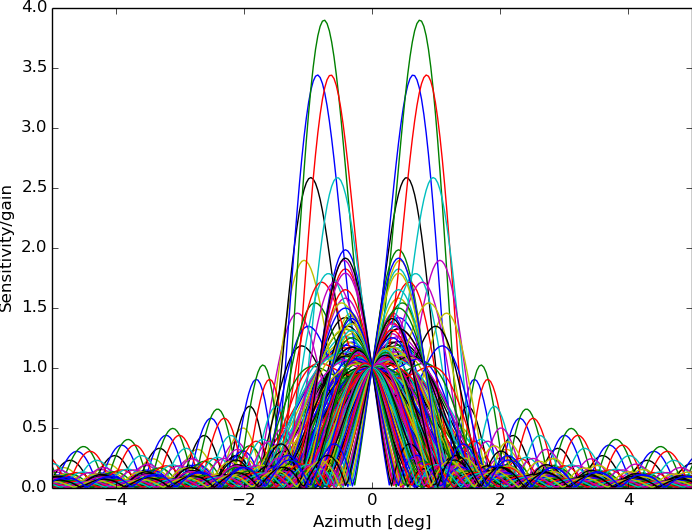
\includegraphics[width=0.49\linewidth]{gfx/6_window_response.png}}\hfill
\subfloat[Mean images]{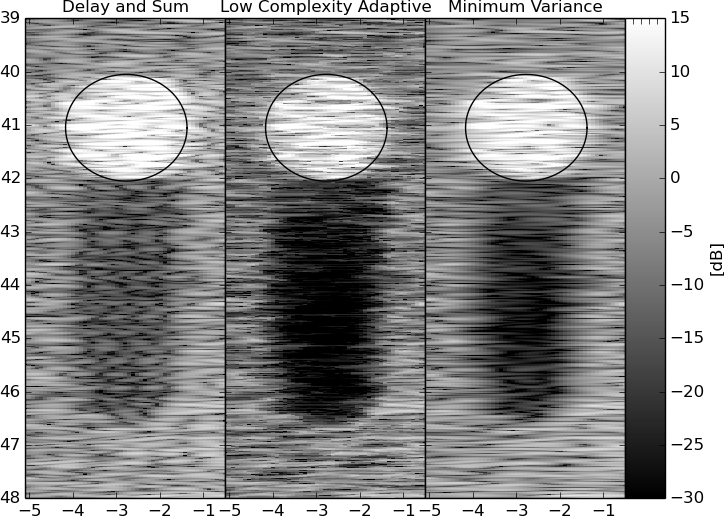
\includegraphics[width=0.49\linewidth]{gfx/6_mean_imgs.png}}\\
\subfloat[Windows ($\beta$)]{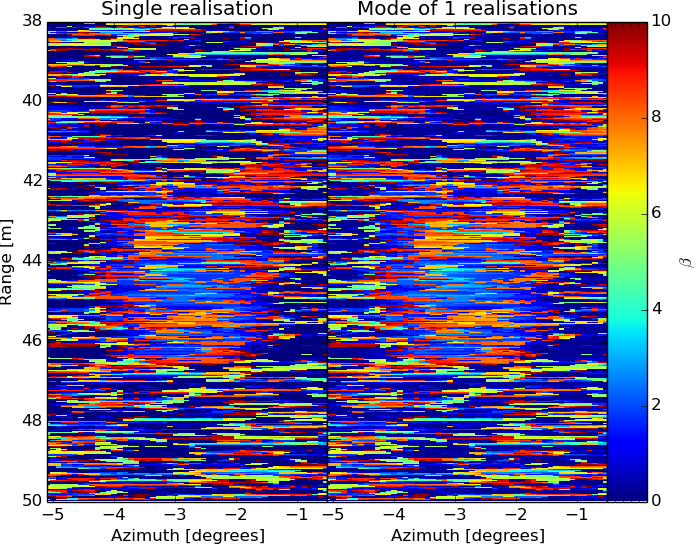
\includegraphics[width=0.49\linewidth]{gfx/6_windows_beta.png}}\hfill
\subfloat[Windows ($\phi$)]{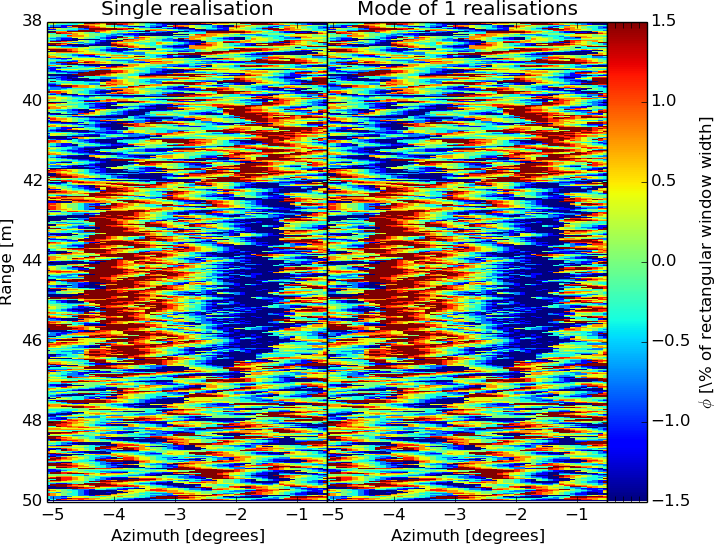
\includegraphics[width=0.48\linewidth]{gfx/6_windows_phi.png}}\\
\subfloat[Capon win. resp. through shadow]{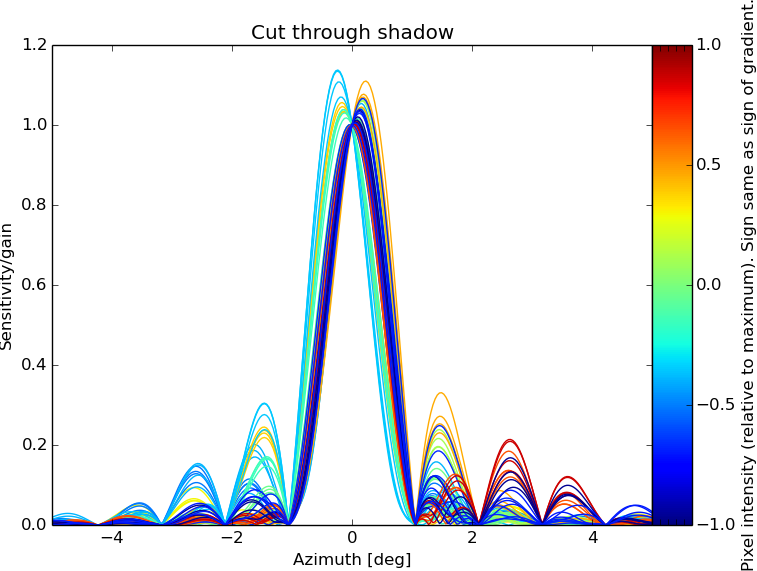
\includegraphics[width=0.49\linewidth]{gfx/6_win_resp_cut_shadow.png}}\hfill
\subfloat[Capon win. resp. through highlight]{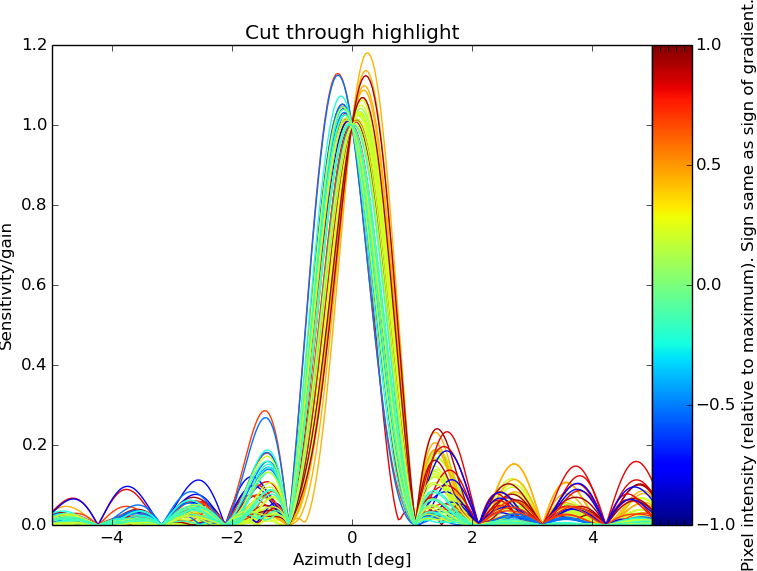
\includegraphics[width=0.49\linewidth]{gfx/6_win_resp_cut_highlight.png}}\\
\end{narrow}
\end{figure*}
\newpage
\begin{figure*}[!t]
\begin{narrow}{-1.2cm}{-1.2cm}\centering\vspace{-1.0cm}
\textbf{7. Capon: Tuning time averaging.}\\
\begin{tabular}[c]{l l l l}
\bf General & M = 32                            & $\Delta r = \frac{c}{2B}$ = 2.5 cm & $\frac{640\,\text{pixels}] / 12\,\text{m}}{\Delta r} = \frac{4}{3}$ \\
\bf LCA     & $\beta \in [0,10]$ (9 values) & $\phi \in [-1.07,1.07]$ deg (9 values) & Navg = 1 \\
\bf Capon   & $\Delta$ = 0.01                 & L = 16                           & Navg = 1 \\
\end{tabular}
\subfloat[LCA Window Response]{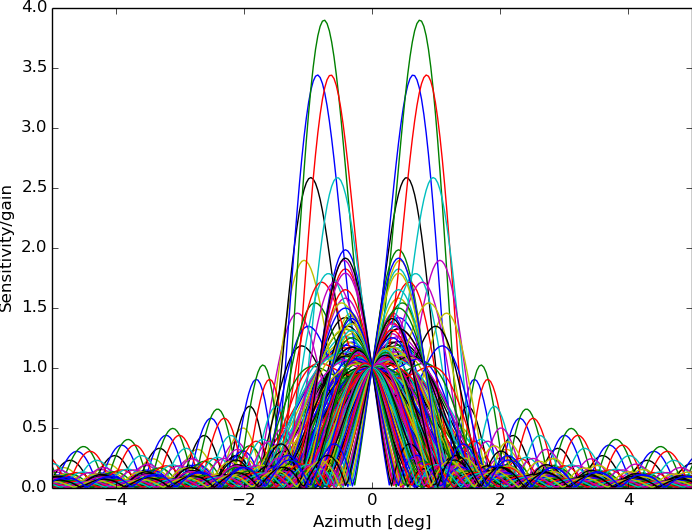
\includegraphics[width=0.49\linewidth]{gfx/7_window_response.png}}\hfill
\subfloat[Mean images]{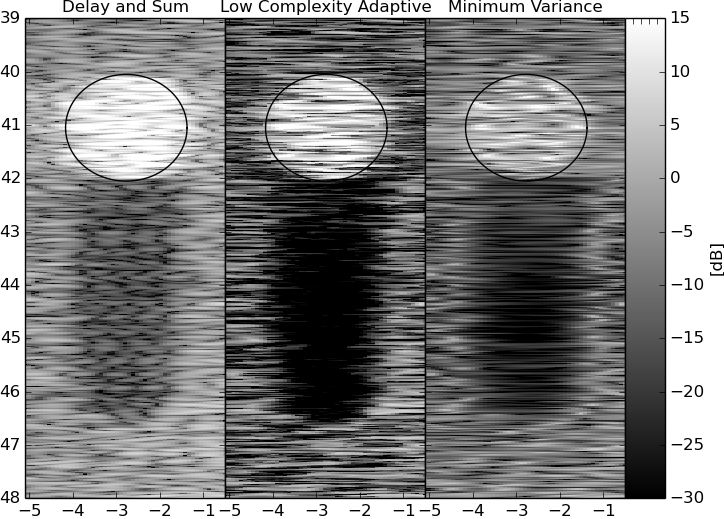
\includegraphics[width=0.49\linewidth]{gfx/7_mean_imgs.png}}\\
\subfloat[Windows ($\beta$)]{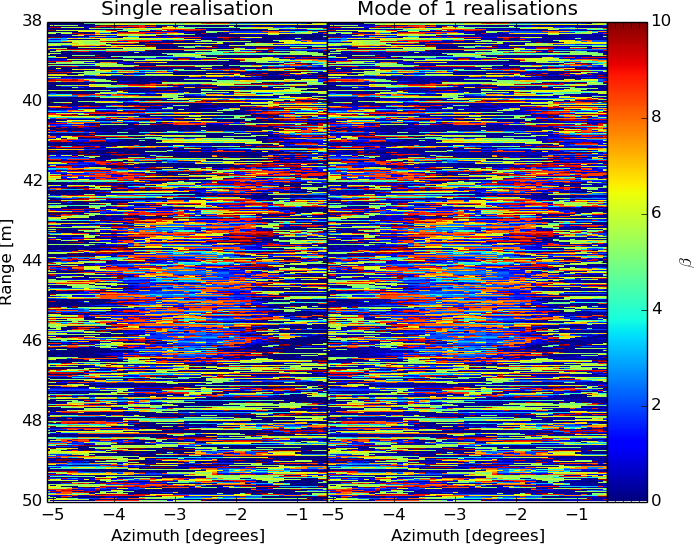
\includegraphics[width=0.49\linewidth]{gfx/7_windows_beta.png}}\hfill
\subfloat[Windows ($\phi$)]{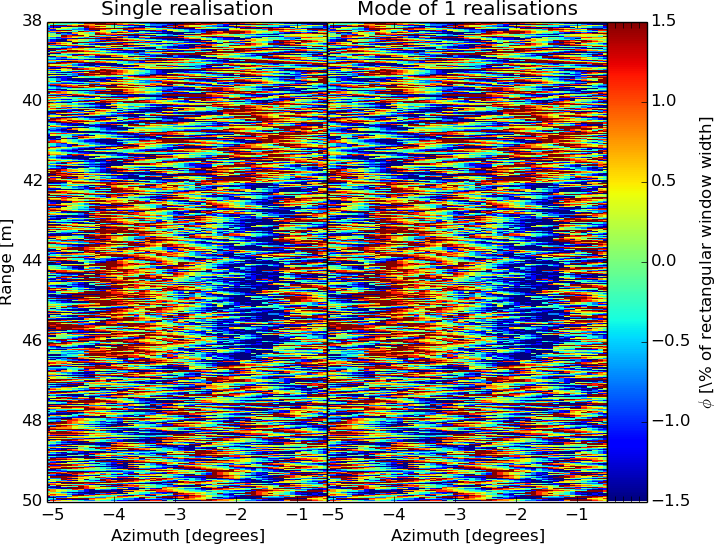
\includegraphics[width=0.48\linewidth]{gfx/7_windows_phi.png}}\\
\subfloat[Capon win. resp. through shadow]{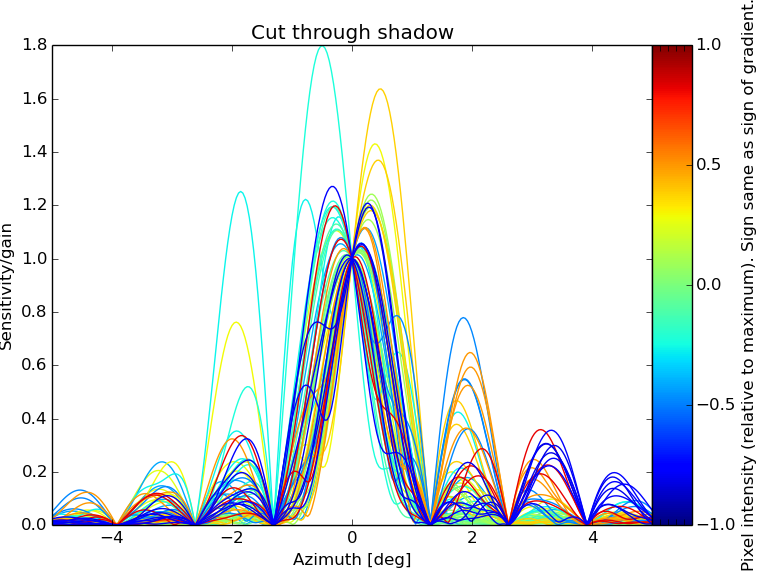
\includegraphics[width=0.49\linewidth]{gfx/7_win_resp_cut_shadow.png}}\hfill
\subfloat[Capon win. resp. through highlight]{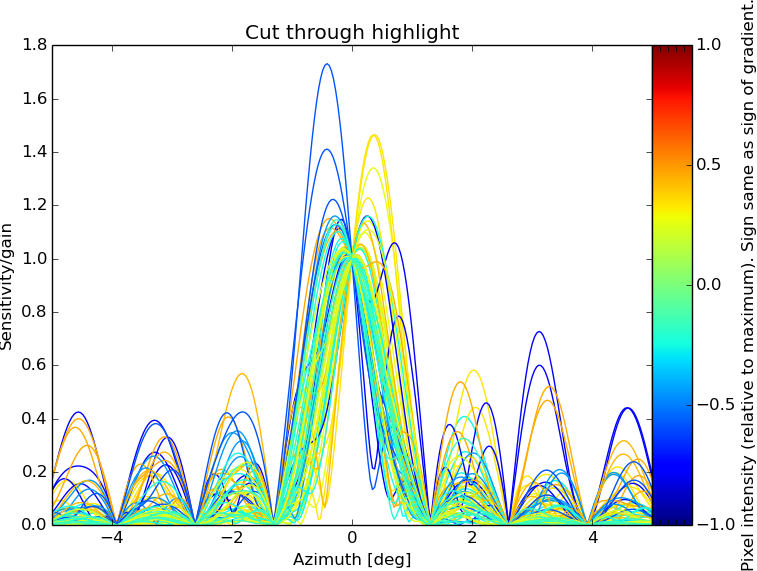
\includegraphics[width=0.49\linewidth]{gfx/7_win_resp_cut_highlight.png}}\\
\end{narrow}
\end{figure*}
\newpage
\begin{figure*}[!t]
\begin{narrow}{-1.2cm}{-1.2cm}\centering\vspace{-1.0cm}
\textbf{8. Capon: Tuning time averaging.}\\
\begin{tabular}[c]{l l l l}
\bf General & M = 32                            & $\Delta r = \frac{c}{2B}$ = 2.5 cm & $\frac{640\,\text{pixels}] / 12\,\text{m}}{\Delta r} = \frac{4}{3}$ \\
\bf LCA     & $\beta \in [0,10]$ (9 values) & $\phi \in [-1.07,1.07]$ deg (9 values) & Navg = 3 \\
\bf Capon   & $\Delta$ = 0.01                 & L = 16                           & Navg = 3 \\
\end{tabular}
\subfloat[LCA Window Response]{\includegraphics[width=0.49\linewidth]{gfx/8_window_response.png}}\hfill
\subfloat[Mean images]{\includegraphics[width=0.49\linewidth]{gfx/8_mean_imgs.png}}\\
\subfloat[Windows ($\beta$)]{\includegraphics[width=0.49\linewidth]{gfx/8_windows_beta.png}}\hfill
\subfloat[Windows ($\phi$)]{\includegraphics[width=0.48\linewidth]{gfx/8_windows_phi.png}}\\
\subfloat[Capon win. resp. through shadow]{\includegraphics[width=0.49\linewidth]{gfx/8_win_resp_cut_shadow.png}}\hfill
\subfloat[Capon win. resp. through highlight]{\includegraphics[width=0.49\linewidth]{gfx/8_win_resp_cut_highlight.png}}\\
\end{narrow}
\end{figure*}
\newpage
\begin{figure*}[!t]
\begin{narrow}{-1.2cm}{-1.2cm}\centering\vspace{-1.0cm}
\textbf{9. Capon: Tuning time averaging.}\\
\begin{tabular}[c]{l l l l}
\bf General & M = 32                            & $\Delta r = \frac{c}{2B}$ = 2.5 cm & $\frac{640\,\text{pixels}] / 12\,\text{m}}{\Delta r} = \frac{4}{3}$ \\
\bf LCA     & $\beta \in [0,10]$ (9 values) & $\phi \in [-1.07,1.07]$ deg (9 values) & Navg = 5 \\
\bf Capon   & $\Delta$ = 0.01                 & L = 16                           & Navg = 5 \\
\end{tabular}
\subfloat[LCA Window Response]{\includegraphics[width=0.49\linewidth]{gfx/9_window_response.png}}\hfill
\subfloat[Mean images]{\includegraphics[width=0.49\linewidth]{gfx/9_mean_imgs.png}}\\
\subfloat[Windows ($\beta$)]{\includegraphics[width=0.49\linewidth]{gfx/9_windows_beta.png}}\hfill
\subfloat[Windows ($\phi$)]{\includegraphics[width=0.48\linewidth]{gfx/9_windows_phi.png}}\\
\subfloat[Capon win. resp. through shadow]{\includegraphics[width=0.49\linewidth]{gfx/9_win_resp_cut_shadow.png}}\hfill
\subfloat[Capon win. resp. through highlight]{\includegraphics[width=0.49\linewidth]{gfx/9_win_resp_cut_highlight.png}}\\
\end{narrow}
\end{figure*}
\newpage
\begin{figure*}[!t]
\begin{narrow}{-1.2cm}{-1.2cm}\centering\vspace{-1.0cm}
\textbf{10. Capon: Tuning time averaging.}\\
\begin{tabular}[c]{l l l l}
\bf General & M = 32                            & $\Delta r = \frac{c}{2B}$ = 2.5 cm & $\frac{640\,\text{pixels}] / 12\,\text{m}}{\Delta r} = \frac{4}{3}$ \\
\bf LCA     & $\beta \in [0,10]$ (9 values) & $\phi \in [-1.07,1.07]$ deg (9 values) & Navg = 7 \\
\bf Capon   & $\Delta$ = 0.01                 & L = 16                           & Navg = 7 \\
\end{tabular}
\subfloat[LCA Window Response]{\includegraphics[width=0.49\linewidth]{gfx/10_window_response.png}}\hfill
\subfloat[Mean images]{\includegraphics[width=0.49\linewidth]{gfx/10_mean_imgs.png}}\\
\subfloat[Windows ($\beta$)]{\includegraphics[width=0.49\linewidth]{gfx/10_windows_beta.png}}\hfill
\subfloat[Windows ($\phi$)]{\includegraphics[width=0.48\linewidth]{gfx/10_windows_phi.png}}\\
\subfloat[Capon win. resp. through shadow]{\includegraphics[width=0.49\linewidth]{gfx/10_win_resp_cut_shadow.png}}\hfill
\subfloat[Capon win. resp. through highlight]{\includegraphics[width=0.49\linewidth]{gfx/10_win_resp_cut_highlight.png}}\\
\end{narrow}
\end{figure*}
\newpage
\begin{figure*}[!t]
\begin{narrow}{-1.2cm}{-1.2cm}\centering\vspace{-1.0cm}
\textbf{11. LCA: Reasonable settings.}\\
\begin{tabular}[c]{l l l l}
\bf General & M = 32                            & $\Delta r = \frac{c}{2B}$ = 2.5 cm & $\frac{640\,\text{pixels}] / 12\,\text{m}}{\Delta r} = \frac{4}{3}$ \\
\bf LCA     & $\beta \in [0,10]$ (9 values) & $\phi \in [-0.57,0.57]$ deg (9 values) & Navg = 7 \\
\bf Capon   & $\Delta$ = 0.01                 & L = 16                           & Navg = 7 \\
\end{tabular}
\subfloat[LCA Window Response]{\includegraphics[width=0.49\linewidth]{gfx/11_window_response.png}}\hfill
\subfloat[Mean images]{\includegraphics[width=0.49\linewidth]{gfx/11_mean_imgs.png}}\\
\subfloat[Windows ($\beta$)]{\includegraphics[width=0.49\linewidth]{gfx/11_windows_beta.png}}\hfill
\subfloat[Windows ($\phi$)]{\includegraphics[width=0.48\linewidth]{gfx/11_windows_phi.png}}\\
\subfloat[Capon win. resp. through shadow]{\includegraphics[width=0.49\linewidth]{gfx/11_win_resp_cut_shadow.png}}\hfill
\subfloat[Capon win. resp. through highlight]{\includegraphics[width=0.49\linewidth]{gfx/11_win_resp_cut_highlight.png}}\\
\end{narrow}
\end{figure*}
\newpage
\begin{figure*}[!t]
\begin{narrow}{-1.2cm}{-1.2cm}\centering\vspace{-1.0cm}
\textbf{12. LCA: Lots of Kaiser windows - wide span.}\\
\begin{tabular}[c]{l l l l}
\bf General & M = 32                            & $\Delta r = \frac{c}{2B}$ = 2.5 cm & $\frac{640\,\text{pixels}] / 12\,\text{m}}{\Delta r} = \frac{4}{3}$ \\
\bf LCA     & $\beta \in [0,20]$ (19 values) & $\phi \in [-1.07,1.07]$ deg (19 values) & Navg = 7 \\
\bf Capon   & $\Delta$ = 0.01                 & L = 16                           & Navg = 7 \\
\end{tabular}
\subfloat[LCA Window Response]{\includegraphics[width=0.49\linewidth]{gfx/12_window_response.png}}\hfill
\subfloat[Mean images]{\includegraphics[width=0.49\linewidth]{gfx/12_mean_imgs.png}}\\
\subfloat[Windows ($\beta$)]{\includegraphics[width=0.49\linewidth]{gfx/12_windows_beta.png}}\hfill
\subfloat[Windows ($\phi$)]{\includegraphics[width=0.48\linewidth]{gfx/12_windows_phi.png}}\\
\subfloat[Capon win. resp. through shadow]{\includegraphics[width=0.49\linewidth]{gfx/12_win_resp_cut_shadow.png}}\hfill
\subfloat[Capon win. resp. through highlight]{\includegraphics[width=0.49\linewidth]{gfx/12_win_resp_cut_highlight.png}}\\
\end{narrow}
\end{figure*}
\newpage
\begin{figure*}[!t]
\begin{narrow}{-1.2cm}{-1.2cm}\centering\vspace{-1.0cm}
\textbf{13. LCA: Lots of trigonometric windows - wide span.}\\
\begin{tabular}[c]{l l l l}
\bf General & M = 32                            & $\Delta r = \frac{c}{2B}$ = 2.5 cm & $\frac{640\,\text{pixels}] / 12\,\text{m}}{\Delta r} = \frac{4}{3}$ \\
\bf LCA     & $\beta \in [0,20]$ (19 values) & $\phi \in [-1.07,1.07]$ deg (19 values) & Navg = 7 \\
\bf Capon   & $\Delta$ = 0.01                 & L = 16                           & Navg = 7 \\
\end{tabular}
\subfloat[LCA Window Response]{\includegraphics[width=0.49\linewidth]{gfx/13_window_response.png}}\hfill
\subfloat[Mean images]{\includegraphics[width=0.49\linewidth]{gfx/13_mean_imgs.png}}\\
\subfloat[Windows ($\beta$)]{\includegraphics[width=0.49\linewidth]{gfx/13_windows_beta.png}}\hfill
\subfloat[Windows ($\phi$)]{\includegraphics[width=0.48\linewidth]{gfx/13_windows_phi.png}}\\
\subfloat[Capon win. resp. through shadow]{\includegraphics[width=0.49\linewidth]{gfx/13_win_resp_cut_shadow.png}}\hfill
\subfloat[Capon win. resp. through highlight]{\includegraphics[width=0.49\linewidth]{gfx/13_win_resp_cut_highlight.png}}\\
\end{narrow}
\end{figure*}
\newpage
\begin{figure*}[!t]
\begin{narrow}{-1.2cm}{-1.2cm}\centering\vspace{-1.0cm}
\textbf{14. LCA: Back on Kaiser - reducing steering span.}\\
\begin{tabular}[c]{l l l l}
\bf General & M = 32                            & $\Delta r = \frac{c}{2B}$ = 2.5 cm & $\frac{640\,\text{pixels}] / 12\,\text{m}}{\Delta r} = \frac{4}{3}$ \\
\bf LCA     & $\beta \in [0,20]$ (19 values) & $\phi \in [-0.72,0.72]$ deg (19 values) & Navg = 7 \\
\bf Capon   & $\Delta$ = 0.01                 & L = 16                           & Navg = 7 \\
\end{tabular}
\subfloat[LCA Window Response]{\includegraphics[width=0.49\linewidth]{gfx/14_window_response.png}}\hfill
\subfloat[Mean images]{\includegraphics[width=0.49\linewidth]{gfx/14_mean_imgs.png}}\\
\subfloat[Windows ($\beta$)]{\includegraphics[width=0.49\linewidth]{gfx/14_windows_beta.png}}\hfill
\subfloat[Windows ($\phi$)]{\includegraphics[width=0.48\linewidth]{gfx/14_windows_phi.png}}\\
\subfloat[Capon win. resp. through shadow]{\includegraphics[width=0.49\linewidth]{gfx/14_win_resp_cut_shadow.png}}\hfill
\subfloat[Capon win. resp. through highlight]{\includegraphics[width=0.49\linewidth]{gfx/14_win_resp_cut_highlight.png}}\\
\end{narrow}
\end{figure*}
\newpage
\begin{figure*}[!t]
\begin{narrow}{-1.2cm}{-1.2cm}\centering\vspace{-1.0cm}
\textbf{15. LCA: Reducing steering span.}\\
\begin{tabular}[c]{l l l l}
\bf General & M = 32                            & $\Delta r = \frac{c}{2B}$ = 2.5 cm & $\frac{640\,\text{pixels}] / 12\,\text{m}}{\Delta r} = \frac{4}{3}$ \\
\bf LCA     & $\beta \in [0,20]$ (19 values) & $\phi \in [-0.36,0.36]$ deg (19 values) & Navg = 7 \\
\bf Capon   & $\Delta$ = 0.01                 & L = 16                           & Navg = 7 \\
\end{tabular}
\subfloat[LCA Window Response]{\includegraphics[width=0.49\linewidth]{gfx/15_window_response.png}}\hfill
\subfloat[Mean images]{\includegraphics[width=0.49\linewidth]{gfx/15_mean_imgs.png}}\\
\subfloat[Windows ($\beta$)]{\includegraphics[width=0.49\linewidth]{gfx/15_windows_beta.png}}\hfill
\subfloat[Windows ($\phi$)]{\includegraphics[width=0.48\linewidth]{gfx/15_windows_phi.png}}\\
\subfloat[Capon win. resp. through shadow]{\includegraphics[width=0.49\linewidth]{gfx/15_win_resp_cut_shadow.png}}\hfill
\subfloat[Capon win. resp. through highlight]{\includegraphics[width=0.49\linewidth]{gfx/15_win_resp_cut_highlight.png}}\\
\end{narrow}
\end{figure*}
\newpage
\begin{figure*}[!t]
\begin{narrow}{-1.2cm}{-1.2cm}\centering\vspace{-1.0cm}
\textbf{16. LCA: Adjusting resolution/SNR.}\\
\begin{tabular}[c]{l l l l}
\bf General & M = 32                            & $\Delta r = \frac{c}{2B}$ = 2.5 cm & $\frac{640\,\text{pixels}] / 12\,\text{m}}{\Delta r} = \frac{4}{3}$ \\
\bf LCA     & $\beta \in [0,5]$ (19 values) & $\phi \in [-0.72,0.72]$ deg (19 values) & Navg = 7 \\
\bf Capon   & $\Delta$ = 0.01                 & L = 16                           & Navg = 7 \\
\end{tabular}
\subfloat[LCA Window Response]{\includegraphics[width=0.49\linewidth]{gfx/16_window_response.png}}\hfill
\subfloat[Mean images]{\includegraphics[width=0.49\linewidth]{gfx/16_mean_imgs.png}}\\
\subfloat[Windows ($\beta$)]{\includegraphics[width=0.49\linewidth]{gfx/16_windows_beta.png}}\hfill
\subfloat[Windows ($\phi$)]{\includegraphics[width=0.48\linewidth]{gfx/16_windows_phi.png}}\\
\subfloat[Capon win. resp. through shadow]{\includegraphics[width=0.49\linewidth]{gfx/16_win_resp_cut_shadow.png}}\hfill
\subfloat[Capon win. resp. through highlight]{\includegraphics[width=0.49\linewidth]{gfx/16_win_resp_cut_highlight.png}}\\
\end{narrow}
\end{figure*}
\newpage
\begin{figure*}[!t]
\begin{narrow}{-1.2cm}{-1.2cm}\centering\vspace{-1.0cm}
\textbf{17. LCA: Adjusting resolution/SNR.}\\
\begin{tabular}[c]{l l l l}
\bf General & M = 32                            & $\Delta r = \frac{c}{2B}$ = 2.5 cm & $\frac{640\,\text{pixels}] / 12\,\text{m}}{\Delta r} = \frac{4}{3}$ \\
\bf LCA     & $\beta \in [5,20]$ (19 values) & $\phi \in [-0.72,0.72]$ deg (19 values) & Navg = 7 \\
\bf Capon   & $\Delta$ = 0.01                 & L = 16                           & Navg = 7 \\
\end{tabular}
\subfloat[LCA Window Response]{\includegraphics[width=0.49\linewidth]{gfx/17_window_response.png}}\hfill
\subfloat[Mean images]{\includegraphics[width=0.49\linewidth]{gfx/17_mean_imgs.png}}\\
\subfloat[Windows ($\beta$)]{\includegraphics[width=0.49\linewidth]{gfx/17_windows_beta.png}}\hfill
\subfloat[Windows ($\phi$)]{\includegraphics[width=0.48\linewidth]{gfx/17_windows_phi.png}}\\
\subfloat[Capon win. resp. through shadow]{\includegraphics[width=0.49\linewidth]{gfx/17_win_resp_cut_shadow.png}}\hfill
\subfloat[Capon win. resp. through highlight]{\includegraphics[width=0.49\linewidth]{gfx/17_win_resp_cut_highlight.png}}\\
\end{narrow}
\end{figure*}
\newpage
\begin{figure*}[!t]
\begin{narrow}{-1.2cm}{-1.2cm}\centering\vspace{-1.0cm}
\textbf{18. LCA: Fewer windows.}\\
\begin{tabular}[c]{l l l l}
\bf General & M = 32                            & $\Delta r = \frac{c}{2B}$ = 2.5 cm & $\frac{640\,\text{pixels}] / 12\,\text{m}}{\Delta r} = \frac{4}{3}$ \\
\bf LCA     & $\beta \in [0,10]$ (9 values) & $\phi \in [-0.72,0.72]$ deg (19 values) & Navg = 7 \\
\bf Capon   & $\Delta$ = 0.01                 & L = 16                           & Navg = 7 \\
\end{tabular}
\subfloat[LCA Window Response]{\includegraphics[width=0.49\linewidth]{gfx/18_window_response.png}}\hfill
\subfloat[Mean images]{\includegraphics[width=0.49\linewidth]{gfx/18_mean_imgs.png}}\\
\subfloat[Windows ($\beta$)]{\includegraphics[width=0.49\linewidth]{gfx/18_windows_beta.png}}\hfill
\subfloat[Windows ($\phi$)]{\includegraphics[width=0.48\linewidth]{gfx/18_windows_phi.png}}\\
\subfloat[Capon win. resp. through shadow]{\includegraphics[width=0.49\linewidth]{gfx/18_win_resp_cut_shadow.png}}\hfill
\subfloat[Capon win. resp. through highlight]{\includegraphics[width=0.49\linewidth]{gfx/18_win_resp_cut_highlight.png}}\\
\end{narrow}
\end{figure*}
\newpage
\begin{figure*}[!t]
\begin{narrow}{-1.2cm}{-1.2cm}\centering\vspace{-1.0cm}
\textbf{19. LCA: Fewer steering angles.}\\
\begin{tabular}[c]{l l l l}
\bf General & M = 32                            & $\Delta r = \frac{c}{2B}$ = 2.5 cm & $\frac{640\,\text{pixels}] / 12\,\text{m}}{\Delta r} = \frac{4}{3}$ \\
\bf LCA     & $\beta \in [0,10]$ (19 values) & $\phi \in [-0.72,0.72]$ deg (9 values) & Navg = 7 \\
\bf Capon   & $\Delta$ = 0.01                 & L = 16                           & Navg = 7 \\
\end{tabular}
\subfloat[LCA Window Response]{\includegraphics[width=0.49\linewidth]{gfx/19_window_response.png}}\hfill
\subfloat[Mean images]{\includegraphics[width=0.49\linewidth]{gfx/19_mean_imgs.png}}\\
\subfloat[Windows ($\beta$)]{\includegraphics[width=0.49\linewidth]{gfx/19_windows_beta.png}}\hfill
\subfloat[Windows ($\phi$)]{\includegraphics[width=0.48\linewidth]{gfx/19_windows_phi.png}}\\
\subfloat[Capon win. resp. through shadow]{\includegraphics[width=0.49\linewidth]{gfx/19_win_resp_cut_shadow.png}}\hfill
\subfloat[Capon win. resp. through highlight]{\includegraphics[width=0.49\linewidth]{gfx/19_win_resp_cut_highlight.png}}\\
\end{narrow}
\end{figure*}
\newpage
\begin{figure*}[!t]
\begin{narrow}{-1.2cm}{-1.2cm}\centering\vspace{-1.0cm}
\textbf{20. LCA: Fewer both.}\\
\begin{tabular}[c]{l l l l}
\bf General & M = 32                            & $\Delta r = \frac{c}{2B}$ = 2.5 cm & $\frac{640\,\text{pixels}] / 12\,\text{m}}{\Delta r} = \frac{4}{3}$ \\
\bf LCA     & $\beta \in [0,10]$ (9 values) & $\phi \in [-0.72,0.72]$ deg (9 values) & Navg = 7 \\
\bf Capon   & $\Delta$ = 0.01                 & L = 16                           & Navg = 7 \\
\end{tabular}
\subfloat[LCA Window Response]{\includegraphics[width=0.49\linewidth]{gfx/20_window_response.png}}\hfill
\subfloat[Mean images]{\includegraphics[width=0.49\linewidth]{gfx/20_mean_imgs.png}}\\
\subfloat[Windows ($\beta$)]{\includegraphics[width=0.49\linewidth]{gfx/20_windows_beta.png}}\hfill
\subfloat[Windows ($\phi$)]{\includegraphics[width=0.48\linewidth]{gfx/20_windows_phi.png}}\\
\subfloat[Capon win. resp. through shadow]{\includegraphics[width=0.49\linewidth]{gfx/20_win_resp_cut_shadow.png}}\hfill
\subfloat[Capon win. resp. through highlight]{\includegraphics[width=0.49\linewidth]{gfx/20_win_resp_cut_highlight.png}}\\
\end{narrow}
\end{figure*}
\newpage
\begin{figure*}[!t]
\begin{narrow}{-1.2cm}{-1.2cm}\centering\vspace{-1.0cm}
\textbf{21. LCA: Even less.}\\
\begin{tabular}[c]{l l l l}
\bf General & M = 32                            & $\Delta r = \frac{c}{2B}$ = 2.5 cm & $\frac{640\,\text{pixels}] / 12\,\text{m}}{\Delta r} = \frac{4}{3}$ \\
\bf LCA     & $\beta \in [0,5]$ (9 values) & $\phi \in [-0.72,0.72]$ deg (5 values) & Navg = 7 \\
\bf Capon   & $\Delta$ = 0.01                 & L = 16                           & Navg = 7 \\
\end{tabular}
\subfloat[LCA Window Response]{\includegraphics[width=0.49\linewidth]{gfx/21_window_response.png}}\hfill
\subfloat[Mean images]{\includegraphics[width=0.49\linewidth]{gfx/21_mean_imgs.png}}\\
\subfloat[Windows ($\beta$)]{\includegraphics[width=0.49\linewidth]{gfx/21_windows_beta.png}}\hfill
\subfloat[Windows ($\phi$)]{\includegraphics[width=0.48\linewidth]{gfx/21_windows_phi.png}}\\
\subfloat[Capon win. resp. through shadow]{\includegraphics[width=0.49\linewidth]{gfx/21_win_resp_cut_shadow.png}}\hfill
\subfloat[Capon win. resp. through highlight]{\includegraphics[width=0.49\linewidth]{gfx/21_win_resp_cut_highlight.png}}\\
\end{narrow}
\end{figure*}
\newpage
\begin{figure*}[!t]
\begin{narrow}{-1.2cm}{-1.2cm}\centering\vspace{-1.0cm}
\textbf{22. LCA: Hardly any.}\\
\begin{tabular}[c]{l l l l}
\bf General & M = 32                            & $\Delta r = \frac{c}{2B}$ = 2.5 cm & $\frac{640\,\text{pixels}] / 12\,\text{m}}{\Delta r} = \frac{4}{3}$ \\
\bf LCA     & $\beta \in [0,5]$ (5 values) & $\phi \in [-0.72,0.72]$ deg (5 values) & Navg = 7 \\
\bf Capon   & $\Delta$ = 0.01                 & L = 16                           & Navg = 7 \\
\end{tabular}
\subfloat[LCA Window Response]{\includegraphics[width=0.49\linewidth]{gfx/22_window_response.png}}\hfill
\subfloat[Mean images]{\includegraphics[width=0.49\linewidth]{gfx/22_mean_imgs.png}}\\
\subfloat[Windows ($\beta$)]{\includegraphics[width=0.49\linewidth]{gfx/22_windows_beta.png}}\hfill
\subfloat[Windows ($\phi$)]{\includegraphics[width=0.48\linewidth]{gfx/22_windows_phi.png}}\\
\subfloat[Capon win. resp. through shadow]{\includegraphics[width=0.49\linewidth]{gfx/22_win_resp_cut_shadow.png}}\hfill
\subfloat[Capon win. resp. through highlight]{\includegraphics[width=0.49\linewidth]{gfx/22_win_resp_cut_highlight.png}}\\
\end{narrow}
\end{figure*}


\end{document}


